\chapter{Reconstruction of physics objects}
    \label{chapter:ReconstructionOfObjects}

This chapter describes the reconstruction of the main physics objects that are relevant for the analyses presented in this dissertation.
The identification, reconstruction and calibration of electrons, muons, jets, $b$-jets and missing transverse energy is discussed in detail.
A brief description of the systematic uncertainties associated with these physics objects is also included.

\section{Tracks}
%Rewrite, stolen from Francesco
In the solenoidal magnetic field of the ID,
a charged particle moves along a helicoidal trajectory with
a curvature inversely proportional to its momentum. 
Tracks are the reconstruction of these trajectories from the 
electric signals induced in the detectors.
Therefore, tracks are used to identify charged particles and 
measure their momenta. 
In addition, the extrapolation of the trajectories allows
the identification of the interaction vertices and the reconstruction of decays of long-lived particles such as $b$-hadrons.

Several pattern recognition algorithms~\cite{Cornelissen:1020106} are used to find tracks in the ID.
The tracks typically used in physics analyses are found using an \textit{inside-out} pattern recognition algorithm, which starts building track ``seeds'' considering space points in the silicon detectors and then extending the track candidate 
outwards to the TRT. An \textit{outside-in} sequence, also referred to as back-tracking, takes into account all the hits not considered by the previous algorithm. It is seeded in the TRT and the track candidate is then extrapolated to the silicon detectors.

A reconstructed track is fully specified by the following parameters:
\begin{equation}
( d_0 , z_0 , \phi , \theta , q/p) 
\end{equation}
where $d_0$ and $z_0$ represent the minimum distance to the center of the detector in the transverse plane and in the longitudinal direction respectively. The azimutal and the polar angle are denoted by $\phi$ and $\theta$ respectively, and $q/p$ represents the charge over momentum. Impact parameters and direction are often expressed with respect to the main primary vertex in the event.

\section{Primary vertices}
Due to the large number of protons per bunch crossing, multiple interaction vertices can be reconstructed in the event.
Primary vertices are reconstructed from the combination of reconstructed
tracks with an adaptive vertex fitting algorithm~\cite{ATLAS-CONF-2010-069}
and they are constrained to lie within the estimated position of the beam spot.\footnote{The beam spot is defined as the spatial region around the interaction point where the profiles of the two beams overlap.}

In order to improve the resolution on the vertex spatial position, only vertices that have at least five tracks with $\pT>500 \MeV$ associated with them are considered.
The number of reconstructed primary vertices is used as a measure of the in-time \pileup\ and several calibration parameters depend on it.

The vertex with the highest sum of the squared track $\pT$ is assumed to be the main vertex of the event corresponding to the hardest $\pp$ interaction. 
The rest of the primary vertices are considered \pileup\ interactions.
Vertices incompatible with the beam collision region are considered secondary vertices, also referred to as displaced vertices.
%They typically originate from decays of long-lived particles. 
The reconstruction of secondary vertices is useful to identify $b$- and $c$-hadrons, as it will be described in section~\ref{sec:btagging}.
%The kinematics of the physics objects
%are then recomputed considering this vertex as a new reference point.

\section{Leptons}
\label{sec:Leptons}
The reconstruction and identification of electrons and muons will be discussed.
Tau-lepton reconstruction is not considered since they will not explicitly be used in any of the analyses described in this dissertation.
Although no attempt is made to identify the tau-leptons, their decay products can still contribute to the object reconstruction.
Leptonic tau decays can be identified as isolated electrons or muons, whereas hadronic tau decays are reconstructed as narrow jets in the detector.

\subsection{Electrons}
    \label{subsec:Electrons}
    Electron candidates are built by searching for a narrow, localized cluster of energy in the EM calorimeter, with at least one ID track associated to it~\cite{Aad:2014fxa}. A sliding-window clustering algorithm~\cite{Lampl:2008zz} is used to identify electron clusters. The algorithm performs a scan of the calorimeter, searching for local maxima of energy within a window of dimensions $3 \times 5$ in units of $0.025\times0.025$ in $\Delta \eta \times \Delta \phi$ space.

Tracks from the inner detector are extrapolated to the middle layer of the electromagnetic calorimeter and matched to the cluster seed. The absolute value of $\Delta\eta$ between the cluster and the track, $|\Delta\eta|$, has to be smaller than $0.05$.  The $\Delta\phi$ must satisfy the relationship $ -0.05 < q\cdot\Delta\phi < 0.10 $. The sign-corrected $\Delta\phi$ selection takes into account the bending direction of the electron in the solenoidal magnetic field.
Matched clusters are then rebuilt with a slightly larger window, $3\times7$ or $5\times5$, depending on whether they are located in the barrel or in the end-cap.

The electron four-momentum is built from the cluster energy and the direction of the associated ID track.
The final cluster energy is obtained by correcting for the energy losses in the material in front of the calorimeter, the lateral leakage due to the fixed cluster size and the longitudinal leakage in the hadronic calorimeter.
Such corrections are derived from detailed studies in MC simulation, test beams and ${Z \rightarrow e^+e^-}$ data events~\cite{Aad:2014nim}.

Electron identification is performed on the candidate electrons in order to suppress the mis-identification of other particles. 
Different conditions on cluster shape are applied, using the fact that the shower development is narrower for electrons than for hadrons, and the hadronic leakage is smaller. 
Track-quality requirements reduce the impact of accidental track association with photons, energetic $\pi^0$ or $\rho$ mesons with electromagnetic decays that can be reconstructed as a single energy cluster. 

Three reference selections have been produced with increasing background rejection: \textit{loose}, \textit{medium} and \textit{tight}. 
Figure~\ref{fig:OBeleID} shows the comparison of the efficiency for each benchmark selection~\cite{EGAMMAsf}. The identification efficiencies depend on the electron $\et$ and pseudo–rapidity, while they are not strongly affected by \pileup. The efficiencies are measured using the ``tag-and-probe'' method.
This method selects a clean and unbiased sample of leptons (probe) from $Z$ boson
decays using selection cuts on one of the leptons in the decay
(tag). The efficiency is determined by applying the selection to the probe lepton.
The modeling in simulation differs slightly from what is observed in data, therefore a calibration scale factor is applied in MC samples.

\begin{figure}[tb!]
\centering
\begin{subfigure}[b]{0.49\textwidth}
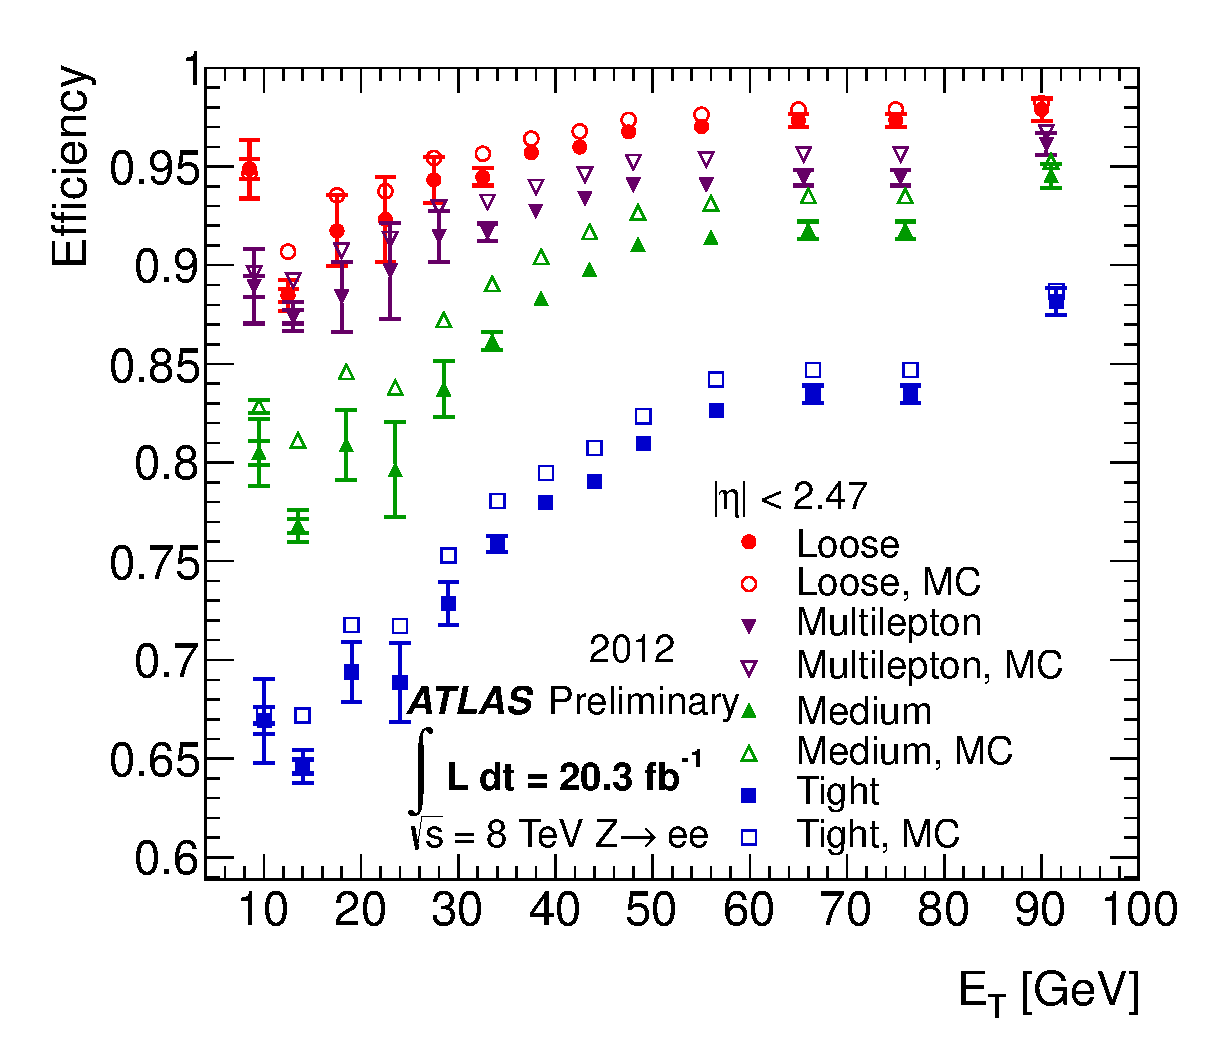
\includegraphics[width=\textwidth]{Objects/Figures/Fig5a_electronid_et.eps}
\caption{}
\end{subfigure}
\begin{subfigure}[b]{0.49\textwidth}
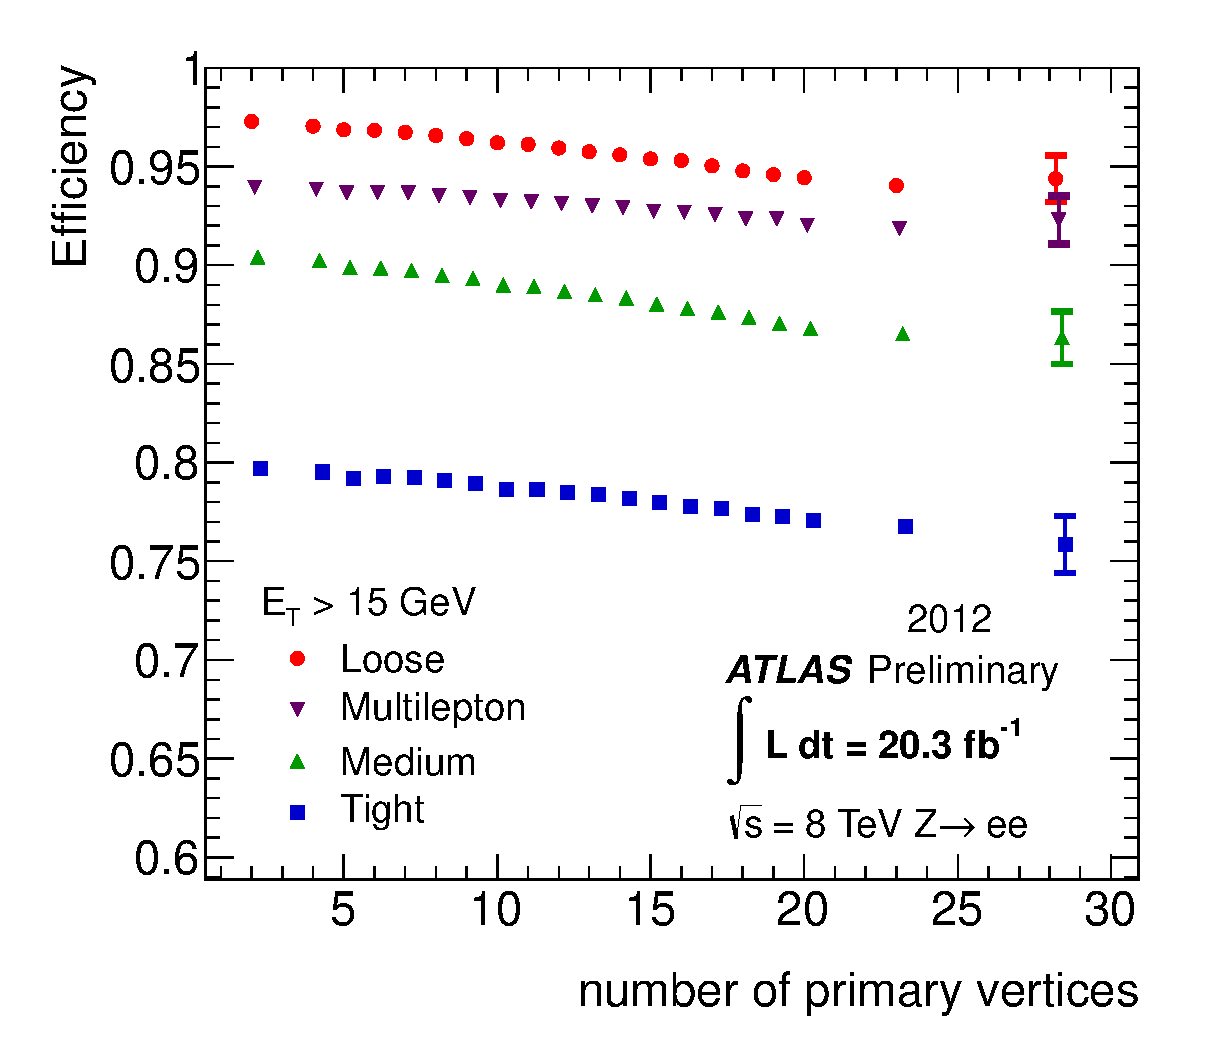
\includegraphics[width=\textwidth]{Objects/Figures/Fig7a_electronid_npv.eps}
\caption{}
\end{subfigure}
\caption{ (a) Electron identification efficiency as a function on electron \ET\ for the benchmark selections in data and MC. 
(b) Measured electron identification efficiency in data for the different benchmark selection as a function of the number of reconstructed primary vertices in the event. 
}
\label{fig:OBeleID}
\end{figure} 

Finally, an additional isolation requirement can be applied to reject electrons from semi-leptonic decays of heavy hadrons. 
The track isolation variable $\pT^{R}$ is defined as the sum of the transverse momenta of all the tracks in a cone of radius $R$ around the electron direction. Only tracks with $\pT > 1 \GeV$ and compatible with being originated from the primary vertex are considered
with the exception of the track used to build the electron object. 
The calorimetric isolation variable called $\ET^{R}$ represents the sum of the transverse energy of the calorimetric cells in the cone of radius $R$ around the electron with the deposit associated with the electron itself subtracted.
%Additional corrections are applied to improve the performance of the calorimetric isolation~\cite{EGAMMAiso}. 
%Due to the fixed size of the electron cluster, higher-energy clusters tend not to be fully contained and, as a net effect, the isolation energy increases as a function of the electron \pT\ even for well isolated electrons. 
%A \pT-leakage correction is derived from MC to compensate for this effect.
%In order to compensate for the \pileup\ effect, an ambient energy density (ED-correction) subtraction is applied. This technique is very similar to the one used for the jet calibration and will be further discussed in the jet section.
The variables  $\ET^{0.2}$ and $\pT^{0.3}$ have been chosen, 
%This stems from the fact that, even after the \pileup\ suppression, smaller cone sizes are preferable due to the topology of \ttbar\ events where jets are likely to be found closer to the selected electrons. %%% \cor{(need to expand?)}.
%The cut values were chosen in order to obtain a constant efficiency of 90\% as a function of \pT\ and $\eta$ for real electrons already fulfilling the \textit{tight} identification criteria.
with variable cut values in order to obtain a constant efficiency of 90\% as a function of \pT\ and $\eta$ for real electrons already fulfilling the \textit{tight} identification criteria.

The analyses presented in this dissertation use the \textit{tight} electron definition since they require the largest possible rejection of ``fake'' electrons from mis-identifications. 
Electrons are required to have $|\eta_{\rm cluster}|<2.47$ and to be 
outside the transition region between the barrel and end-cap 
EM calorimeter ($1.37<|\eta_{\rm cluster}|<1.52$)
since this region shows worse reconstruction and energy 
resolution performance.
Finally, electron isolation is required to reject electrons from semileptonic hadron decays.

%The \textit{tight} selection has an efficiency of $\sim$ 80\% for electrons coming from $Z$ decay with a rejection against jets faking electron of $10^5$ as estimated from MC samples~\cite{ELECTRONpub}.

A different electron definition, with looser selection criteria, will also be used to estimate the contribution of multijet events where a jet is reconstructed as an electron. This looser definition uses \textit{medium} as identification criteria, no isolation requirement, and a veto on the conversion of a photon into electrons by requiring a hit in the innermost ID layer. The use of this looser electron set will be described in detail in section~\ref{subsec:QCD}.

%\subsubsection{Reconstruction, identification and isolation cut uncertainties}
The efficiency of the reconstruction, identification and isolation selection has been determined in data using the tag-and-probe method using $Z\rightarrow \eebar$ events, which provide high-statistics and high-purity samples of electrons. Samples of selected $J/\psi\rightarrow \eebar$ and $W\rightarrow e\nu_e$ events are also used in order to collect sufficient statistics for a two-dimensional $\pt-\eta$ identification efficiency determination. 
%For the reconstruction efficiency measurement, $Z\rightarrow \eebar$ events have been used since they allow for the purest selection of probes.
%To assess the identification efficiency, a combined analysis using $J/\psi\rightarrow \eebar$, $Z\rightarrow \eebar$ and $W\rightarrow e\nu_e$ 
%events has been performed to cover as wide a \pt\ range as possible and collect sufficient statistics for a 2D $\pt-\eta$ efficiency determination.
%The isolation efficiency for the electrons satisfying the tight identification criteria has been also assessed using $Z\rightarrow \eebar$ events.

Scale factors as a function of electron $\eta$ and electron \ET\ have been derived to account for the discrepancies in the efficiencies between data and MC simulation.
These scale factors typically deviate from unity by only a few \%. 
The combined uncertainties on the reconstruction, identification and isolation requirement scale factors are at the level of $\sim \unit[2]{\%}$.
For \ttbar-related analyses, an additional uncertainty of \unit[2]{\%} is assumed for the isolation efficiency, due to the extrapolation from the $Z\rightarrow \eebar$ environment 
to the \ttbar\ environment, involving higher jet multiplicity and therefore smaller angular separation between the electron and surrounding jets~\cite{TOPRECO8TeV}.

\subsubsection{Electron energy scale and resolution}
The electron energy scale has been measured in data using $Z\rightarrow \eebar$ and $J/\psi\rightarrow \eebar$ events.
Correction factors as a function of the electron $\eta$ have been obtained by fitting the dielectron invariant mass distributions of the two resonances.
The total uncertainty on the electron in-situ calibration is $< 1\%$ in the central region and increases up to a few \% in the most forward region of the calorimeter.
An additional procedure, exploiting the combined measurement of the track momentum in the inner detector and the energy in the calorimeter ($E/p$) has also been used, profiting from the very large sample of collected $W\rightarrow e\nu_{e}$ events.
%The two analyses have been widely used to monitor the azimuthal uniformity of the calorimeter response, the \pT-linearity and the stability over time and \pileup\ conditions.

The main way to probe the electron energy resolution is provided by the study of the $Z$ resonance width.
It is found that the resolution in data is slightly worse than
that in simulation, and appropriate corrections are
derived and applied to simulation to match the data.

\subsection{Muons}
    \label{subsec:Muons}
Several types of algorithms for reconstructing muons are available in ATLAS~\cite{Aad:2014rra}. 
The analyses presented in this dissertation make use only of \textit{combined} muons from the \textit{MuId} collection.
The algorithm relies on the independent reconstruction of a track in the Inner Detector and a track segment in the muon spectrometer. A combined track is formed after re-fitting the hits of both tracks, taking into account the muon energy loss in the calorimeter.
%All track pairs with a small $\Delta R$ distance are considered and
%combined muons are then identified by a common track re-fit to the hits of both tracks, taking into account the muon energy loss in the calorimeter. %\footnote{the algorithm allows also for other hits to be included in the fitting procedure}. 
%This fit has high rejection power against mismatches between inner detector and stand-alone muon tracks.

Additional selection criteria are applied to further improve the quality of the muon and reduce the misidentification rate: %% (put reference): can I quote a twiki??
\begin{itemize}
\item Combined muons are required to have $|\eta| < 2.5$ in order to be confined to the region with ID coverage.
\item The longitudinal impact parameter relative to the primary vertex is required to be less than \unit[2]{mm}.
\item A minimal number of hits in the Pixel, SCT and TRT sub-detectors is required, together with a hit in the innermost pixel layer when the track
  crosses an active module.
\end{itemize}

A further separation between prompt muons arising from the hard interaction and muons originating from decay chains of $b/c$-hadrons or kaons, is achieved through an isolation requirement.
The mini-isolation variable, $I^\mu_{mini}$, is introduced. 
It is defined as the sum of the transverse momentum of all the tracks
satisfying the relation $\Delta R_{(\mu, track)} < \unit[10]{\gev}/\pT^\mu$ where $\pT^\mu$ is the transverse momentum of the muon. A selection cut on this variable is applied, corresponding to:
\begin{equation}
I^\mu_{mini} /  \pT^\mu <0.05~.  %%I^\mu_{mini}= \sum_{tracks} \pT^{track} / \pT^\mu < 0.05
\end{equation}

With increasing lepton \pt, the cut on the mini-isolation is relaxed, 
while at the same time the size of the considered cone shrinks making the isolation cut less susceptible to \pileup\ effects and more efficient when the real lepton is close to a jet. 
Figure~\ref{fig:OBmini} shows the signal efficiency vs fake rate curves for different isolation definitions, extracted from $Z\rightarrow \mumubar$ events and a multijet-enriched control region. The relative mini isolation exhibits a superior performance with respect to the usual isolation variables $\ET^{0.2}$ and $\pt^{0.3}$.

\begin{figure}[tb!]
\begin{center}
\includegraphics[width=0.66\textwidth]{Objects/Figures/effrej2.pdf}
\caption{Efficiency vs fake rate for different choices of muon isolation: $\ET^{0.2}$ with a fixed value of $\pt^{0.3}<\unit[2.5]{\gev}$ (red), $\pt^{0.3}$ with a fixed value of $\ET^{0.2}<\unit[4]{\gev}$ (blue), $I^\mu_{mini}$ (yellow) and $I^\mu_{mini} /  \pT^\mu$ (green). Typical working point choices used in 2011 analyses (cross: $\ET^{0.2}<\unit[4]{\gev}$ and $\pt^{0.3}<\unit[2.5]{\gev}$) and 2012 analyses (star: $I^\mu_{mini} /  \pT^\mu <0.05$) are also indicated. From reference~\protect\cite{TOPRECO8TeV_pre}.}
\label{fig:OBmini}
\end{center}
\end{figure} 

A second muon definition, with looser selection criteria, will also be used to estimate the contribution from non-prompt muons arising from semi-leptonic hadron decays.
This looser definition removes the isolation requirement in order to increase the contribution from multijet events. The use of this second set of muons will be described in detail in section~\ref{subsec:QCD}.


%\subsubsection{Reconstruction, identification and isolation uncertainties}
The reconstruction, identification and isolation efficiencies have been measured in data with the tag-and-probe method using $Z\rightarrow \mumubar$ and $J/\psi \to \mumubar$ events.
Figure~\ref{fig:OBmuID} shows the data/MC comparison for the reconstruction plus identification efficiency and the isolation efficiency.
The level of agreement and the corresponding uncertainties are $\sim$ 1\% and found to be very stable versus other kinematic quantities as well as versus the number of primary vertices in the event. 
\begin{figure}[tb!]
\centering
\begin{subfigure}[t]{0.44\textwidth}
\includegraphics[width=0.99\textwidth]{Objects/Figures/fig_12b__MUONID.pdf}
\caption{}                                            
\end{subfigure}                                       
\begin{subfigure}[t]{0.50\textwidth}                  
\includegraphics[width=0.99\textwidth]{Objects/Figures/effiso_eta.pdf}%should I plot mu?
\caption{}
\end{subfigure}
\caption{ (a) Muon reconstruction+identification efficiency and scale factor as a function of muon $\eta$. (b) Mini Isolation efficiency as a function of muon $\eta$ for data and MC. }
\label{fig:OBmuID}
\end{figure} 

\subsubsection{Muon momentum scale and resolution}
The large number of clean $Z\rightarrow \mumubar$ and $J/\psi \to \mumubar$ events collected allows a simultaneous determination of the muon momentum scale and resolution by performing a fit to the dimuon invariant mass distributions of the $Z$ and $J/\psi$ resonances~\cite{Aad:2014rra}. Correction factors for the momentum scale and resolution are determined separately for the Muon Spectrometer and Inner Detector.
Figure~\ref{fig:OBmuSc} illustrates the central value and the uncertainty of the correction to the muon momentum scale in the Muon Spectrometer.
The amount of the correction, as well as the uncertainty, are at the few per mille level.
\begin{figure}[t!] %t!p
\centering
\includegraphics[width=0.6\textwidth]{Objects/Figures/fig_13b__NEWMUONSCALE.pdf}
\caption{Scale correction for the muon momentum in the muon spectrometer as a function of muon $\eta$.}
\label{fig:OBmuSc}
\end{figure} 
%The muon momentum resolution depends on multiple factors like the amount of material that the muon traverses, the spatial resolution of the individual track points and the quality of the relative alignment of the sub-detectors.
%For this reason, a separate parameterization has been used for the Inner Detector and the Muon Spectrometer part.
%\footnote{the muon \pT\ resolution can be expressed as: 
%$\sigma(\pT)/\pT=a \oplus b\cdot \pT$ where $a$ represents the contribution from multiple scattering and $b$ describes the intrinsic resolution caused by the spatial resolution of the detector components, and any residual misalignment.}

These factors, and their relative uncertainties, are used to correct the MC scaling the muon \pt\ and introducing additional smearing to match the data. Figure~\ref{fig:OBmuRes} shows the di-muon invariant mass for data and MC, before and after such corrections have been applied.

\begin{figure}[tb!] %t!p
\centering
\begin{subfigure}{0.38\textwidth}
\includegraphics[width=\textwidth]{Objects/Figures/fig_14a__lineshapeBefore.pdf}
\caption{}
\end{subfigure}
\begin{subfigure}{0.38\textwidth}
\includegraphics[width=\textwidth]{Objects/Figures/fig_14b__lineshapeAfter.pdf}
\caption{}
\end{subfigure}
\caption{Comparison of di-muon invariant mass in data, before (a) and after (b) MC smearing and scale corrections are applied.}
\label{fig:OBmuRes}
\end{figure} 

\section{Jets}
    \label{sec:JetReco}

    One of the consequences of color confinement is that quarks and gluons produced in the hard interactions can not be found isolated.
    %can not be found/observed isolated
    %making therefore impossible to pro- duce isolated quarks
    %quarks and gluons, which always carry colour charge, cannot appear as free particles.
    Instead they evolve into a spray of collimated particles, in a process called \textit{hadronization}.
    A jet can be defined as a grouping of the particles produced in the hadronization, in order to obtain a physics object whose characteristics are as close as possible to those of the initial parton.

    Different categories of jets can be defined based on the type of inputs and the algorithm used to combine them and build a jet. 
Jets reconstructed from truth stable particles in MC samples are denoted as \textit{particle jets}. Jets built from 
reconstructed tracks in the detector are called \textit{track jets}. %and they are normally used as an additional tool to extract jet quantities.
Finally, the jets most commonly used in ATLAS analyses are built from energy deposits in the calorimeter called \textit{topo-clusters}~\cite{Lampl:2008zz} and are usually referred to as \textit{reconstructed jets} or simply jets.

\subsection{Cluster formation}
    \label{subsec:JetClusterFormation}

The topological clustering algorithm~\cite{Lampl:2008zz} reconstructs three-dimensional clusters of energy deposits in the calorimeters. It is designed to follow the shower development of a single particle interacting with the calorimeter, taking advantage of the calorimeters' fine granularity.

Seed cells are built by selecting cells with a significant signal-to-noise ratio of $|S/N|\geq 4$.
The noise is defined as the expected RMS of the electronics noise for the current gain and conditions plus the contribution of \pileup\ added in quadrature.
Neighboring cells in the three dimensions are then added to the cluster if their signal to noise ratio is $|S/N|\geq 2$.
Finally, cells with $|S/N|\geq 0$ in the perimeter are added to the cluster, to ensure that the tails of showers are not discarded.
%, while the higher thresholds for seeds and neighbors effectively suppress both electronics and \pileup\ noise.
Figure \ref{fig:JetClusterFormation} shows a schema of a topological cluster formation.
%In case of particles leading to overlapping showers they can still be separated if they form local maxima in the calorimeter.
%Topo-clusters are defined to be massless and represent three dimensional energy blobs in the calorimeter.

\subsection{Jet-finding algorithm}
    \label{subsec:JetClusteringAlgorithm}

\begin{figure}[tb!]
  \begin{center}
    \begin{subfigure}{0.495\textwidth}
      \includegraphics[width=\textwidth]{Objects/Figures/JetClusterFormation.eps}
      \caption{}\label{fig:JetClusterFormation}
    \end{subfigure}
    \begin{subfigure}{0.495\textwidth}
      \includegraphics[width=\textwidth]{Objects/Figures/JetAntiKt.eps}
      \caption{}\label{fig:JetAntiKt}
    \end{subfigure}
  \end{center}
  \caption{
    (a) Grid representing calorimeter cells, showing topo-cluster formation in the three hadronic layers in the barrel. 
  (b) Illustration of the clustering of jets with the $\akt$ algorithm.
  }
  \label{fig:JetTopoClusterAntiKt}
\end{figure}

A jet-finding algorithm is needed to decided which inputs are aggregated into individual jets. 
The $\akt$ algorithm~\cite{Cacciari:2008gp} is a sequential recombination algorithm, and is the default jet-finding algorithm at the LHC experiments. This algorithm has been chosen for its theoretical properties of infrared and collinear safety~\cite{Salam:2009jx}, and for the fact that it produces rather circular jets in the $\eta-\phi$ plane. %e since the hardest particles are clustered at an early stage.
For all the input constituents, the $\akt$ algorithm computes the quantities:

    \begin{equation}
        d_{ij} = \min\left( \frac{1}{k_{Ti}^{2}}, \frac{1}{k_{Tj}^{2}} \right) \frac{\Delta R_{ij}^{2}}{R^2}~,
        \label{eq:AntiKt_dij}
    \end{equation}
    \begin{equation}
        d_{iB} = \frac{1}{k_{Ti}^{2}}~,
        \label{eq:AntiKt_diB}
    \end{equation}

\noindent where $\Delta R_{ij}^{2} = (\eta_i - \eta_j)^2 + (\phi_i - \phi_j)^2$, $R$ is a parameter of the algorithm that approximately controls the size of the jet and $k_{Ti}$ is the transverse momentum of the constituent $i$.
Here, $d_{ij}$ is the ``distance'' between the constituents $i$ and $j$, while $d_{iB}$ is the distance between the constituent $i$ and the beam, introduced to separate constituents coming from the hard-scatter interaction from those coming from proton remnants.

The $\akt$ jet clustering algorithm proceeds by identifying the smallest of the distances, which corresponds to clustering the most energetic particles first.
If the smallest distance is a $d_{ij}$, it recombines the constituents $i$ and $j$, while if the smallest distance is $d_{iB}$, the algorithm calls $i$ a jet and removes it from the list of constituents.
%The method used to recombine the different constituents is called \emph{recombination scheme}.
%In ATLAS, the $E$-scheme is used, in which the four-momentum of the recombined object is defined by the vectorial sum of the four-momenta of its constituents.
After recombination, the distances are recalculated with the remaining constituents, and the procedure is repeated until no constituents are left.
Figure \ref{fig:JetAntiKt} illustrates the clustering of hard and soft particles into jets when the $\akt$ algorithm is applied.

The analyses described in this dissertation use $\akt$ jets with a radius of $R=0.4$.
%The $\akt$ algorithm defines jets with a well-defined conical shape, thus allowing robust \pileup\ corrections.
%Jets are defined with a minimum transverse momentum threshold $p_T^{\text{jet}}$, used as a scale to separate soft from hard interactions.


\subsection{Jet calibration}
    \label{subsec:JetCalibration}

    The goal of the jet calibration procedure is to correct the energy of the reconstructed jets in the detector to correspond to the one of the truth particle jets. First the input clusters are calibrated, then the reconstructed jet undergoes several corrections to reduce the impact of \pileup\ contamination and recover the energy of the truth particle jets on average.

Topo-clusters are initially reconstructed at the EM scale, which correctly measures the energy in the calorimeter deposited by particles produced in an electromagnetic shower.
These clusters then need to be recalibrated to correctly measure the energy deposited by particles produced in a hadronic shower.
This is done with the local cell signal weighting calibration scheme (LCW)~\cite{Aad:2011he}.
The LCW calibration scheme first classifies topo-clusters as either electromagnetic or hadronic based on the measured energy density and the longitudinal shower depth.
Then, energy corrections are derived according to this classification from single charged and neutral pion MC simulations.
Further dedicated corrections are introduced to correct for detector and reconstruction effects, such as energy lost in uninstrumented regions (dead material) or out-of-cluster leakage.
%address effects of calorimeter non-compensation, signal losses due to noise threshold effects and energy loss in non instrumented regions of the detector close to the cluster. 
The analyses described in this dissertation use jets built from LCW-calibrated clusters, which are also referred to as LCW jets. Jets built from non-calibrated clusters are usually named EM jets.

After jet reconstruction based on calibrated clusters, the calibration scheme for calorimeter jets consists of four steps, illustrated in figure~\ref{fig:jes_calibration} and described in the following sections.

\begin{figure}[tb]
  \centering
  \includegraphics[width=\textwidth]{Objects/Figures/fig_03.pdf}
  \caption{Overview of the ATLAS jet calibration scheme.}
  \label{fig:jes_calibration}
\end{figure}

\subsubsection{\Pileup\ correction} 
The presence of additional \pileup\ activity can distort the measured jet energy. A first correction is performed to account for this, according to equation~\ref{eq:pileup_correction}:
\begin{equation}
\label{eq:pileup_correction}
\pT^{\rm corr} =\pT - \rho\cdot A - \alpha \cdot (N_{PV} -1 ) - \beta \cdot \left<\mu\right>,
\end{equation}
where $\rho$ is the \pileup\ energy density of the event, $\alpha = \frac{\partial \pt}{\partial N_{PV}}$ and $\beta =  \frac{\partial \pt}{\partial \mu}$.
The first term represents the \textit{jet-area correction} which allows a jet-by-jet estimation and subtraction of the energy added to the jet by the \pileup~\cite{TheATLAScollaboration:2013pia}.
The \pileup\ energy density of the event, $\rho$, is defined by the median of the distribution of \pT/A for each jet %in the event 
reconstructed in the central region of the detector. 
The jet area A is computed with the ghost-matching method~\cite{JetArea}.
The additional terms in the formula represent residual corrections that remove the remaining effects for both in-time ($\alpha$) and out-of-time ($\beta$) \pileup.
Figure~\ref{fig:JetPileupCorrection} shows the dependence of jet \pT\ on the number of primary vertices (as a measure of in-time \pileup) and of $\langle \mu \rangle$ (as a measure of out-of-time \pileup) as a function of jet $\eta$, at each step of the correction process.

\begin{figure}[tb!]
  \begin{center}
      \includegraphics[width=0.495\textwidth]{Objects/Figures/JetPileupCorrNPV.eps}
      \includegraphics[width=0.495\textwidth]{Objects/Figures/JetPileupCorrMu.eps}
  \end{center}
  \caption[Dependence of the reconstructed jet $\pt$ on in-time \pileup\ and out-of-time \pileup\ at various correction stages.]{Dependence of the reconstructed jet $\pt$ on in-time \pileup\ (left) and out-of-time \pileup\ (right) at various correction stages.}
  \label{fig:JetPileupCorrection}
\end{figure}

\subsubsection{Origin correction} 
A correction to the calorimeter jet direction is applied in order to make the jet point to the primary event vertex instead of the center of the ATLAS detector. 
%Thereafter, the kinematic observables of each topo-cluster are recalculated.
The energy of the jet remains unchanged. 
This correction improves the angular resolution and results in a small improvement in the jet $\pt$ response.

\subsubsection{Jet energy calibration}

After \pileup\ correction, the jet energy calibration restores the reconstructed jet energy to the energy of the MC particle-level jets.
It corrects for detector effects due to the mis-measurement of the deposited energy, the energy lost in inactive regions of the detector or the energy deposits of particles that are not clustered into the reconstructed jet.

To derive this calibration, all the isolated\footnote{
  A jet is considered isolated when no other jet with $\pt > \unit[7]{GeV}$ is found within a cone of radius $\Delta R = 2.5 R$, where $R = 0.4$ is the jet radius.
}
calorimeter jets that have a matching isolated particle-level jet at $\Delta R=0.3$ are considered.
The jet energy response is the ratio between the energy measured in the reconstructed jets, $E_{\mathrm{LCW}}^j$, and the particle-jet energy, $E_{\mathrm{truth}}^j$.
 Since \pileup\ effects have already been corrected for, the MC samples used to derive the calibration do not include
 multiple proton-proton interactions.
Figure \ref{fig:JetCalibrationResponse} shows the jet energy response as a function of the calibrated jet transverse momentum for different $\eta$-intervals. The correction factor needed for LCW jets is closer to unity than the EM jets since the input topo-clusters have already been calibrated.

\begin{figure}[tb!]
  \begin{center}
      \includegraphics[width=0.495\textwidth]{Objects/Figures/fig_04a_EMJES.pdf}
      \includegraphics[width=0.495\textwidth]{Objects/Figures/fig_04b_LCWJES.pdf}
  \end{center}
  \caption{Average response for jets built from topoclusters at the EM scale (left) and at LCW scale (right). The response is shown separately for various particle-jet energies as function of the jet pseudo-rapidity $|\eta_{\mathrm{det}}|$. Also indicated are the different calorimeter regions.}
  \label{fig:JetCalibrationResponse}
\end{figure}


\subsubsection{In-situ calibration}
    \label{subsubsec:InSituCalibration}

As the last step, the data-to-MC differences are assessed using \emph{in-situ} techniques, which exploit the transverse momentum balance between a jet and well-measured photons, $Z$ bosons or jets.
This calibration is only applied to data, since it aims to restore the energy of the jets reconstructed in data to that from the MC simulation.\footnote{The reconstructed jets from the MC simulations are already calibrated with the LCW+JES scheme, which restores the reconstructed jet energy to that of the particle-level jet in the simulation.}

Central jets are calibrated combining in-situ techniques as $Z$+jets, $\gamma$+jets and multi-jet balance calibration~\cite{Aad:2014bia}. Figure~\ref{fig:JetInSituMeasurements} shows the ratio of the jet response, defined as $\pT^{\rm measured}/\pT^{\rm reference}$, between data and MC.
Forward jets are calibrated using the $\eta$-intercalibration technique. It exploits the \pT-balance between jets in different $\eta$ regions where forward jets are calibrated against central jets whose energy scale can be assessed in a more precise way.

\begin{figure}[tb!]
  \begin{center}
      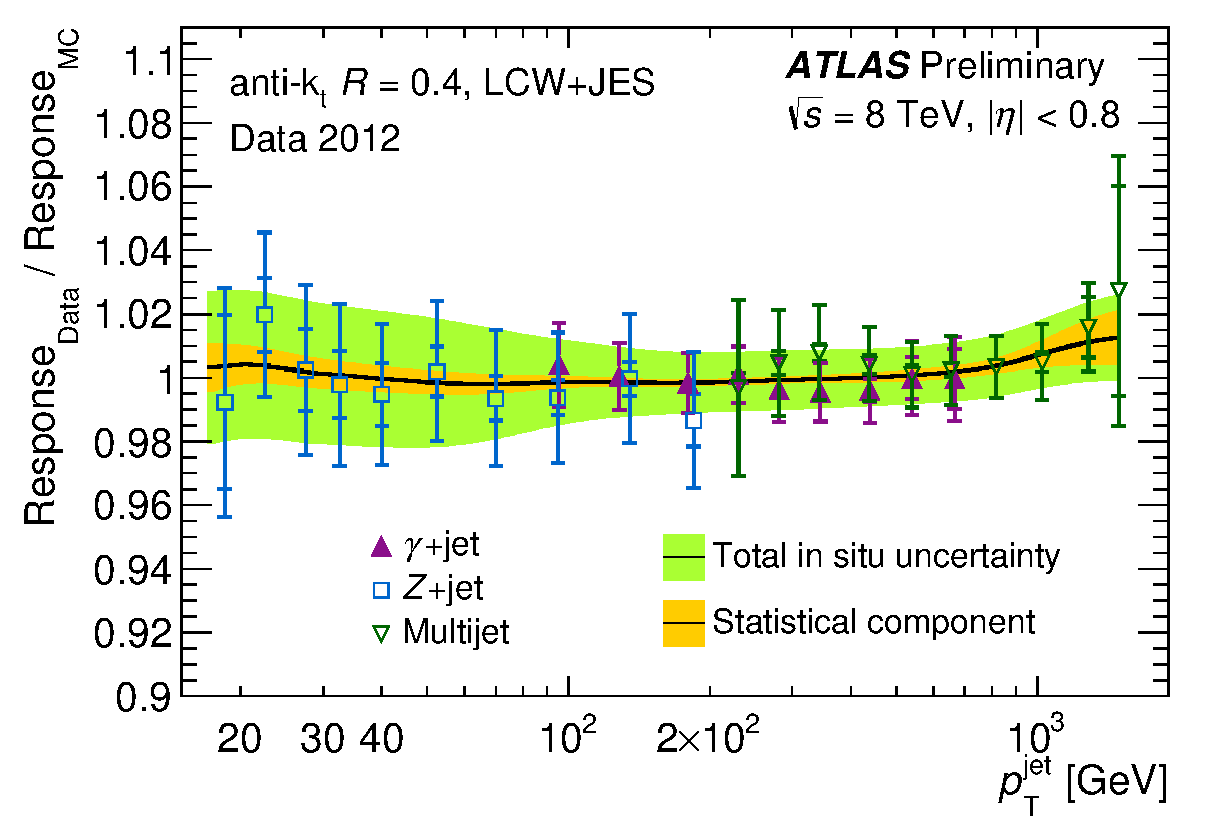
\includegraphics[width=0.7\textwidth]{Objects/Figures/responseRatio_LCJES_R4-2.eps}
  \end{center}
  \caption{Ratio of the average jet response $\langle \pt^{\text{jet}} / \pt^{\text{ref}} \rangle$ measured in data to that measured in MC simulations for jets within $|\eta|<1.2$ as a function of the jet transverse momentum, $\pt^{\text{jet}}$, shown separately for the three in-situ techniques, used in the combined calibration }
  \label{fig:JetInSituMeasurements}
\end{figure}

\subsubsection{Semileptonic $b$-jet corrections}
A further refinement, which is not part of the standard jet calibration, is the correction for semileptonic decays of heavy-flavored hadrons.
In cases when a $b$-hadron decays semileptonically,\footnote{
  The notation \textit{semileptonic} is used to denote any decay chain of the type: $B \rightarrow X+\mu+\nu_{\mu}$. Decays in the electron channel don't require a special treatment since the electron energy is deposited in the calorimeter and clustered into the jet.} the energy of the jet containing that hadron is underestimated since both the muon and the neutrino can carry a substantial part of the hadron energy and they are not considered in the jet clustering process.
Since $b$-hadron decays produce muons in $\sim$ 20\% of the cases (including direct decays and cascade decays via charm-hadrons and $\tau$ leptons), the effect is particularly important for analyses with a large number of $b$-quarks in the final state.
%like the $\ttbar H(H\rightarrow \bbbar)$ final state. 
The jet four-momentum is corrected by combining it with the muon:
\begin{equation}
  \bold{p}_{\rm jet}^{\rm corr}= \bold{p}_{\rm jet} + \sum_i^{\rm muons} ( \bold{p}_{\mu_i} - \bold{E}_{\rm loss}(\mu_i) )
\end{equation}
where $p_{\mu_i}$ is the combined muon and $E_{\rm loss}(\mu_i)$ is the estimated energy loss of the muon in the calorimeter which is subtracted to avoid double-counting.  All muons passing the standard \textit{MuId} selection cut with $\pT> \unit[4]{\GeV}$ and within a distance $\Delta R < 0.4$ to the jet axis are considered in the correction term.

The correction is applied to all jets overlapping with muons, independently of whether they are tagged as $b$-jets. 
The energy losses due to the escaping neutrino are not considered since a correction term was derived based on a different category of muons, \textit{Staco} and not \textit{MuId}, as used in this analysis.
%It has been shown in~\cite{TOPRECO8TeV} that the application of the semi-leptonic correction helps in improving the jet response and \pT\ resolution 
%in case of $b$-quark jets.
Figure~\ref{fig:OBresponse} shows the effect of each correction on a sample of $b$-jets in simulated \ttbar\ events.

\begin{figure}[tb!]
\centering
\begin{subfigure}[t]{0.49\textwidth}
 \includegraphics[width=\textwidth]{Objects/Figures/compSLC_RMS_MS_dptopt_1.pdf}
\caption{}
\end{subfigure}
\begin{subfigure}[t]{0.49\textwidth}
 \includegraphics[width=\textwidth]{Objects/Figures/compSLC_FitGaus_MS_massHadTop_corr_1.pdf}
\caption{}
\end{subfigure}
\caption{  Jet \pT\ resolution (a) and reconstructed hadronic top mass (b) for an inclusive jet sample in MC \ttbar\ events.
The dotted line describes calibrated jets, the dashed line jets after the muon correction and the solid line jets after both the muon and the neutrino corrections.}
\label{fig:OBresponse}
\end{figure} 


\subsection{Jet energy scale uncertainty}
\label{JESunc}
The determination of the jet energy scale uncertainty takes into account multiple sources of systematic uncertainty:
\begin{itemize}
\item Uncertainties due to \pileup\ are assigned to the correction term in equation~\ref{eq:pileup_correction}, to cover the residual mis-modeling of multiple interaction in MC. The impact of the uncertainty rapidly reduces with increasing jet \pT.

\item For very high \pT\ jets ($ \pT > 2 \TeV$) in-situ techniques are limited in statistics. Therefore, studies of detector response based on MC events and extrapolated test-beam results from single-hadron response are used to assess the systematic uncertainty~\cite{Aad:2012vm}. 
  In order to perform this extrapolation, jets are treated as a superposition of energy deposits of single particles. 
  The measurements of the calorimeter response to single pions in the combined test-beam are then extrapolated to high-\pt\ jets.
%In the following they will be referred to as \textit{single particle response}.

\item $\eta$-intercalibration uncertainties are divided into a statistical component and a MC modeling one. They are the dominant source of JES uncertainty at large $\eta$ ($|\eta|>3$). 

\item Uncertainties coming from in-situ techniques are divided in different categories (statistical, detector, modeling, mixed) according to their origin. Particular attention has been paid to preserving the correlation information among the various sources of uncertainty across the different \pT\ bins. The ``diagonalization and reduction'' method has been applied~\cite{Aad:2014bia}. The method identifies the most relevant sources of uncertainty and organizes them into uncorrelated variations which 
can then be applied independently. The remaining (small) sources of uncertainty are grouped together in a residual component.

\item Flavor-related uncertainties: the response of the calorimeter differs for jets initiated by quarks and jets initiated by gluons. In-situ techniques mainly measure quark-initiated jets by the nature of the process involved. The baseline
 uncertainty is then increased using the MC estimates of the response difference between quarks and gluons~\cite{JetFlavDep}. 
% To correctly assess the uncertainty a knowledge of the jets quark/gluon fraction is needed which makes the contribution dependent on the topology under consideration. The uncertainty is evaluated by conservatively assuming a 50\%/50\% mix of quarks and gluons.

\item An additional source of uncertainty in the range of 1.5~\% to 3~\% is considered for jets originating from $b$-quarks. 
The uncertainty has been obtained comparing the jet calibration to an estimate of jet \pT\ performed with track jets
and evaluating the difference between an inclusive jet sample and a sample enriched in jets from $b$-quarks~\cite{JetBJes}.

\end{itemize}

Figure~\ref{fig:OBjes} shows the relative JES uncertainty as a function of jet \pT. The contribution from the different sub categories are also highlighted while the $b$-jet scale uncertainty is not shown. 
The relative JES uncertainty is below 4\% in the whole jet \pT\ range, reaching a precision below 2\% in the range of 100 to \unit[1000]{\GeV}.
 
%This is related to the fact that the energies of all the jets in the event are simultaneously shifted in the same direction.
%For analyses with a refined statistical treatment (profiled likelihood) and dependence on jet kinematics, the usage of multiple uncertainty components is recommended since it allows taking into account the correlation effects correctly, leading to a better estimation of the effect of systematic uncertainties.
 
\begin{figure}[tb!]
\centering
   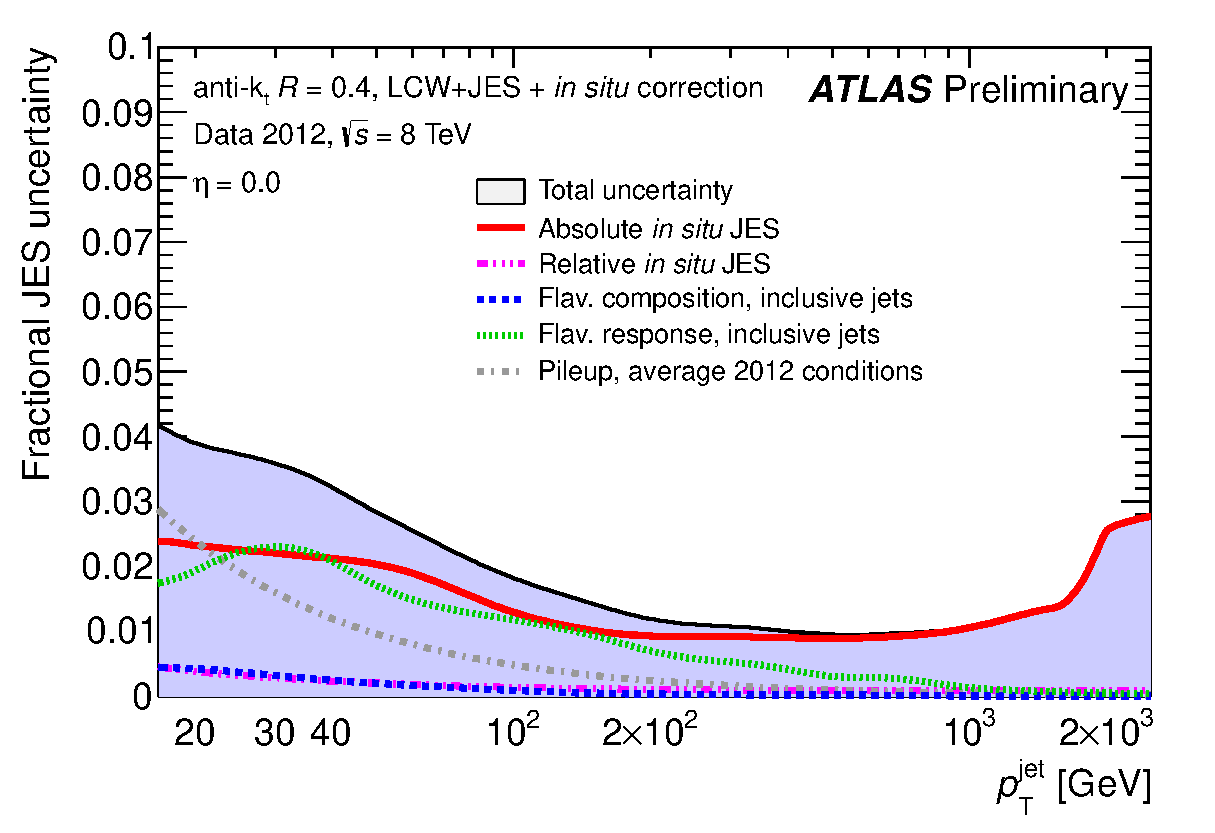
\includegraphics[width=0.6\textwidth]{Objects/Figures/JESUncertainty-Moriond2013-Dijet-LC4-pT-noCloseby.eps}
\caption{Relative jet energy scale uncertainty as a function of \pT\ for central jets in the detector.}
\label{fig:OBjes}
\end{figure}
  
\subsection{Jet energy resolution}
\label{subsec:JER}
The jet energy resolution has been measured in dijet data with the dijet balance and dijet bisector methods~\cite{ATLAS-CONF-2015-017}. 
The dijet balance method uses the imbalance in jet \pt:
\begin{equation}
  \mathcal{A} = \frac{p_{\rm T}^{\rm probe} - p_{\rm T}^{\rm ref} }{p_{\rm T}^{\rm avg}}~,
  \label{eq:jet_asym}
\end{equation}
where $p_{\rm T}^{\rm ref}$ is the transverse momentum of a jet in a well-calibrated reference region, 
$p_{\rm T}^{\rm probe}$ is the transverse momentum of the jet in the calorimeter region under investigation, and 
$p_{\rm T}^{\rm avg} =(p_{\rm T}^{\rm probe} + p_{\rm T}^{\rm ref})/2$.
The jet energy resolution can be extracted with a fit to the width of the asymmetry distribution, $\sigma(\mathcal{A})$.

The dijet bisector method relies on the decomposition of the two leading jet vectorial sum \pT\ in orthogonal directions, one of them being the bi-section of the $\Delta\phi$ angles between the two jets in dijet events. The sensitivity to jet energy resolution is different for the two since in the bisector direction the \pT\ is the sum of two small components while in the orthogonal direction a subtraction of the much larger projection is performed.

The measured values are in reasonable agreement with the MC prediction, as shown in figure~\ref{fig:OBjer}, with some differences in particular regions of the phase space (high $\eta$, high \pT) where the resolution in data has been found to be larger than the expectations.
The effect has been considered as a source of systematic uncertainty where additional smearing of the \pT\ of the simulated jets is applied to cover the difference with data. The resolution has been measured for dijet-\pt\ down to \unit[40]{\gev}, and the uncertainty is estimated for the lower \pt\ region by performing a fit to the measured resolution and extrapolating the uncertainty below the measured the range. 
\begin{figure}[tb!]
\centering
\includegraphics[width=0.7\textwidth]{Objects/Figures/figaux_06a_JER.pdf}
\caption{Comparison of jet energy resolution as a function of jet \pt\ for data and MC in the region $0.0 \leq |\eta_{\rm det}| < 0.8$.}
\label{fig:OBjer}
\end{figure} 


\subsection{Jet reconstruction efficiency}
The jet reconstruction efficiency for calorimeter jets has been derived relative to track-jets, using a tag-and-probe technique. The reconstruction efficiency is defined as the fraction of probe track-jets matched to a calorimeter jet. 
Small differences, $\sim\unit[0.2]{\%}$, are observed between data and MC in the range $\pt < \unit[30]{\GeV}$.  As a source of systematic uncertainty the difference is applied to MC events by discarding a fraction of jets taken at random within the inefficiency range.

\subsection{Jet cleaning and jet vertex fraction}
\label{subsec:cleanJet}
Not all the jets that are reconstructed in detector have their origin in the $\pp$ collisions. 
Transient problems in the calorimeter hardware,
LHC beam-gas interactions or showers induced by cosmic rays can create fake jets, also referred to as ``bad jets''.
Quality criteria are applied to reject such jets:
\begin{itemize}
\item The shape of the electrical signal collected in every calorimeter cell is compared to the reference (quality factor), and a jet quality factor is computed weighting the cell quality with the cell energy squared. Jets with significant deviation from the reference quality factor are rejected. %this is the various HECQ, LArQ
\item The energy of the jet deposited in the electromagnetic calorimeter must be between 5\% and 95\%. This helps reducing noise effects from the EM calorimeter and from non-collision backgrounds.
\item Due to the larger noise in the hadronic endcap calorimeter, the fraction of the jet energy in this subdetector has to be smaller than 50\%.
\item The energy fraction of a jet contained in one single layer of the calorimeter should be smaller than 99\%. 
\end{itemize}
%This selection is also particularly important for the missing transverse energy calculation since the presence of fake jets could give rise to a large \pT\ imbalance.

\Pileup\ activity can also produce jets which should not be considered as part of the hard-scatter event. 
In order to identify and reject in-time \pileup, information from the tracks associated to each jet is used.
The jet vertex fraction (JVF) is a variable aiming to identify the vertex from which a jet is originated~\cite{TheATLAScollaboration:2013pia}. 
It is defined as the ratio of the sum of transverse momentum of matched tracks that originate from a chosen PV to the sum of transverse momentum of all matched tracks in the jet, independently of their origin. 
JVF can be defined for each jet with respect to each PV, and therefore for a given jet $i$, its JVF with respect to the primary vertex $j$, PV$_j$, is given by:

\begin{equation}
\text{JVF}(\text{jet}_i, \text{PV}_j) = \frac{\sum_{k=1}^{N_\text{tracks}}{\pt(\text{track}_{k}^{\text{jet}_i}, \text{PV}_j) }}{ \sum_{n=1}^{N_\text{PV}}{\sum_{k=1}^{N_\text{tracks}}{\pt(\text{track}_{k}^{\text{jet}_i}, \text{PV}_n)} }}.
\label{eq:JetJVFDefinition}
\end{equation}
%The JVF is defined as the sum \pT\ of all tracks from the primary vertex matched to a jet divided by the total jet-matched track \pT\ from all vertices.
%The JVF is defined as the fraction of track coming from the primary vertex out of all the tracks associated to the jet; each track contribution is weighted by its \pT.  
%A track is considered matched to a jet if the angular distance to the jet direction ($\Delta R$) is smaller than 0.4.
The distribution of the JVF for jets originating from the primary (hard scatter) interaction and for \pileup\ originated jets is illustrated in figure~\ref{fig:OBjvf_a}. The JVF variable has a good separation power between hard-scatter jets (peaking at 1)
and \pileup\ jets (having substantially lower fraction of tracks from the primary vertex). A value of -1 is attributed to jets with no associated tracks (mainly at large rapidities).


\begin{figure}[tb!]
\centering
\begin{subfigure}[t]{0.47\textwidth}
   \includegraphics[width=0.99\textwidth]{Objects/Figures/fig_26__JVF.pdf}
\caption{}
\label{fig:OBjvf_a}
\end{subfigure}
\begin{subfigure}[t]{0.37\textwidth}
\includegraphics[width=0.99\textwidth]{Objects/Figures/fig_29__JVF.pdf}
\caption{}
\label{fig:OBjvf_b}
\end{subfigure}
\caption{ (a) JVF distribution for hard-scatter (blue) and \pileup\ (red) jets with 20 $\leq$ \pT $\leq$ 50 \GeV\ and $|\eta| < 2.5$ in simulated Z+jets events. (b) JVF distribution for jets well balanced against $Z\rightarrow \eebar$ candidates 
in data and MC simulation. Plots are taken from reference~\protect\cite{TheATLAScollaboration:2013pia}. }
\label{fig:OBjvf}
\end{figure} 


The cut to suppress \pileup\ jets is defined to be $|\rm{JVF}| >0.50$. This cut gives a 95\% selection efficiency for jets from primary interaction while rejecting 75\% of the \pileup\ jets.  
The cut is applied only to jets with $\pT < 50 \GeV$, since the \pileup\ contribution at high \pT\ is negligible, and with $|\eta|<2.4$, since tracking information is required. 

The effect of the cut has been tested on data and MC using $Z\rightarrow \llbar$ events
where specific selections are applied to obtain a sample of hard-scatter jets and \pileup\ jets.
Figure~\ref{fig:OBjvf_b} displays the comparison between data and MC for a sample enriched in hard-scatter jets.
A systematic uncertainty associated to the JVF selection is estimated by changing the cut values in MC by $\pm 0.03$.

\section{$b$-tagging}
\label{sec:btagging}

The identification of jets resulting from the fragmentation of $b$-quarks, usually referred to as \textit{$b$-tagging}, is of uttermost importance for analyses with high number of $b$-quarks in the final state.
%looking at $H\rightarrow \bbbar$ as well as other interesting physics signals at the LHC.
In the energy regime above \unit[10]{\GeV}, the long lived $b$-hadrons ($\tau\sim$ \unit[1.5]{ps}) produced in the hadronization of $b$-quarks can travel several millimeters, decaying at a sufficiently large distance from the production vertex that a secondary vertex  
can be resolved in the detector (see figure~\ref{fig:OBbtagpic}).
%a given distance from the production vertex thus originating secondary vertices  as show in figure~\ref{fig:OBbtag}.

\begin{figure}[tb!]
\begin{center}
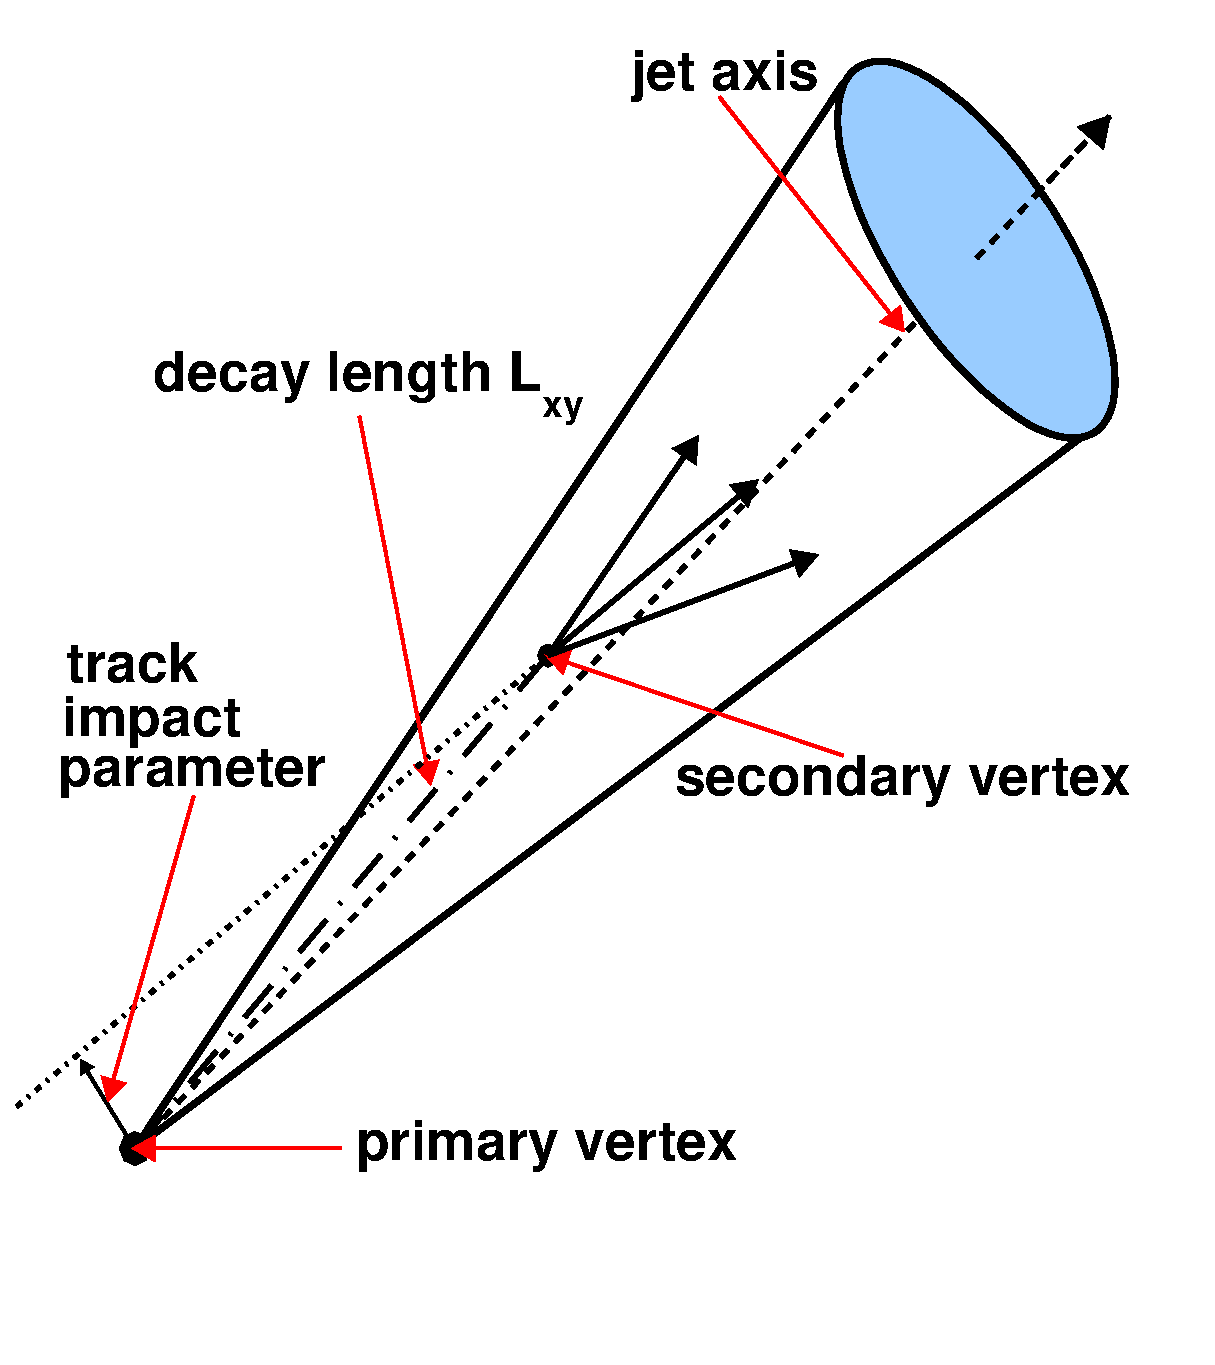
\includegraphics[width=0.5\textwidth]{Objects/Figures/b-jet-sketch.eps}
\caption{Most-relevant variables for the identification of a jet originating from the fragmentation of a $b$-quark.}
\label{fig:OBbtagpic}
\end{center}
\end{figure} 

Several characteristics can be be exploited to identify this signature. 
If the secondary vertex can be identified within a jet, its distance to the primary vertex\footnote{The decay length is divided by its error to obtain the \textit{decay length significance}, $L/\sigma_L$, in order to reduce the effect of poorly-measured vertices.} (\textit{decay length}) as well as the mass of all the particles associated to the vertex can be used for the identification. Secondary vertices from $b$-hadron decays are expected to be significantly displaced from the primary vertex and to have a vertex mass of up to $\sim$ 5 GeV (due to neutral decay products not being included).
Without the need to reconstruct the secondary vertex, the impact parameter of each track in the jet can also be analyzed. The longitudinal and transverse impact parameter are defined as the minimum distance of the track to the primary vertex respectively in the $z$ direction and in the $x$-$y$ plane. 
%The quantities are divided by their error in order to reduce the influence of poorly reconstructed tracks. 
The sign of the impact parameter is positive if the track extrapolation crosses the jet direction in front of the primary vertex, and negative otherwise.
For a jet originating from a $b$-quark, typically one or more tracks are expected to show a large and positive impact parameter significance.

\subsection{$b$-tagging algorithms}
Several algorithms have been developed in ATLAS to perform the $b$-tagging of jets exploiting the properties described before. The most relevant are:
\begin{description}
  \item[IP3D~\cite{HighPerf}:] the longitudinal and transverse impact parameter of the tracks are used in a 2D likelihood ratio discriminant. Input variables are compared to templates for both the $b$-jet and light-jet hypotheses, obtained from MC simulation. 

  \item[SV1~\cite{HighPerf}:] this algorithm relies on the reconstruction of a secondary vertex in the jet. %using tracks fulfilling specific quality criteria. 
    Various variables are combined using a likelihood ratio technique, such as the decay length significance, the invariant mass of all tracks associated with the vertex, the ratio of the sum of the energies of the tracks in the vertex to the sum of the energies of all tracks in the jet, and the number of two-track vertices.

  \item[JetFitter~\cite{JetFitter}:] this algorithm attempts to reconstruct the decay chain inside the jet. A Kalman-fitter approach is used to identify secondary and tertiary vertices with the assumption that they lie on the flight direction of the $b$-hadron.

\item[JetFitterCombNN:] the output of the IP3D and JetFitter algorithms are combined using a neural network in order to improve the discrimination. A different version called JetFitterCombNNc is also available where the neural network is explicitly trained to separate $c$-jets from $b$-jets.

\item[MV1:] the output of the IP3D, SV1 and JetFitterCombNN algorithms are used as input to a neural network. The MV1c algorithm is a particular version of the MV1 algorithm trained to achieve a better separation between jets originating from $b$-quarks and jets originating from $c$-quarks.
\end{description} 

The performance of the algorithms is characterized by their capability to correctly identify jets coming from a real $b$-quark compared to the probability of 
mistakenly $b$-tagging a jet originating from a $c$-quark or a light-flavor parton ($u$, $d$, $s$-quark or gluon). These quantities are commonly referred to as the $c$-tagging efficiency\footnote{
  Dedicated algorithms to identify $c$-jets are also available~\cite{charmtag}. In the context of this dissertation, $c$-tagging refers to mistakenly $b$-tagging a $c$-jet. } 
  and mistag rate respectively.

The $b$-tagging efficiency compared to the light-jet and $c$-jet rejection, is summarized in figure~\ref{fig:OBbtag} for some of the algorithms discussed. The rejection is defined as the inverse of the mistag or $c$-tag rate.
The MV1 algorithm shows the best performance in rejecting light quark jets and is therefore used as the $b$-tagging algorithm of choice for the analyses presented in this dissertation.

\begin{figure}[tb!] %% ht![
\centering
\begin{subfigure}[]{0.40\textwidth}
   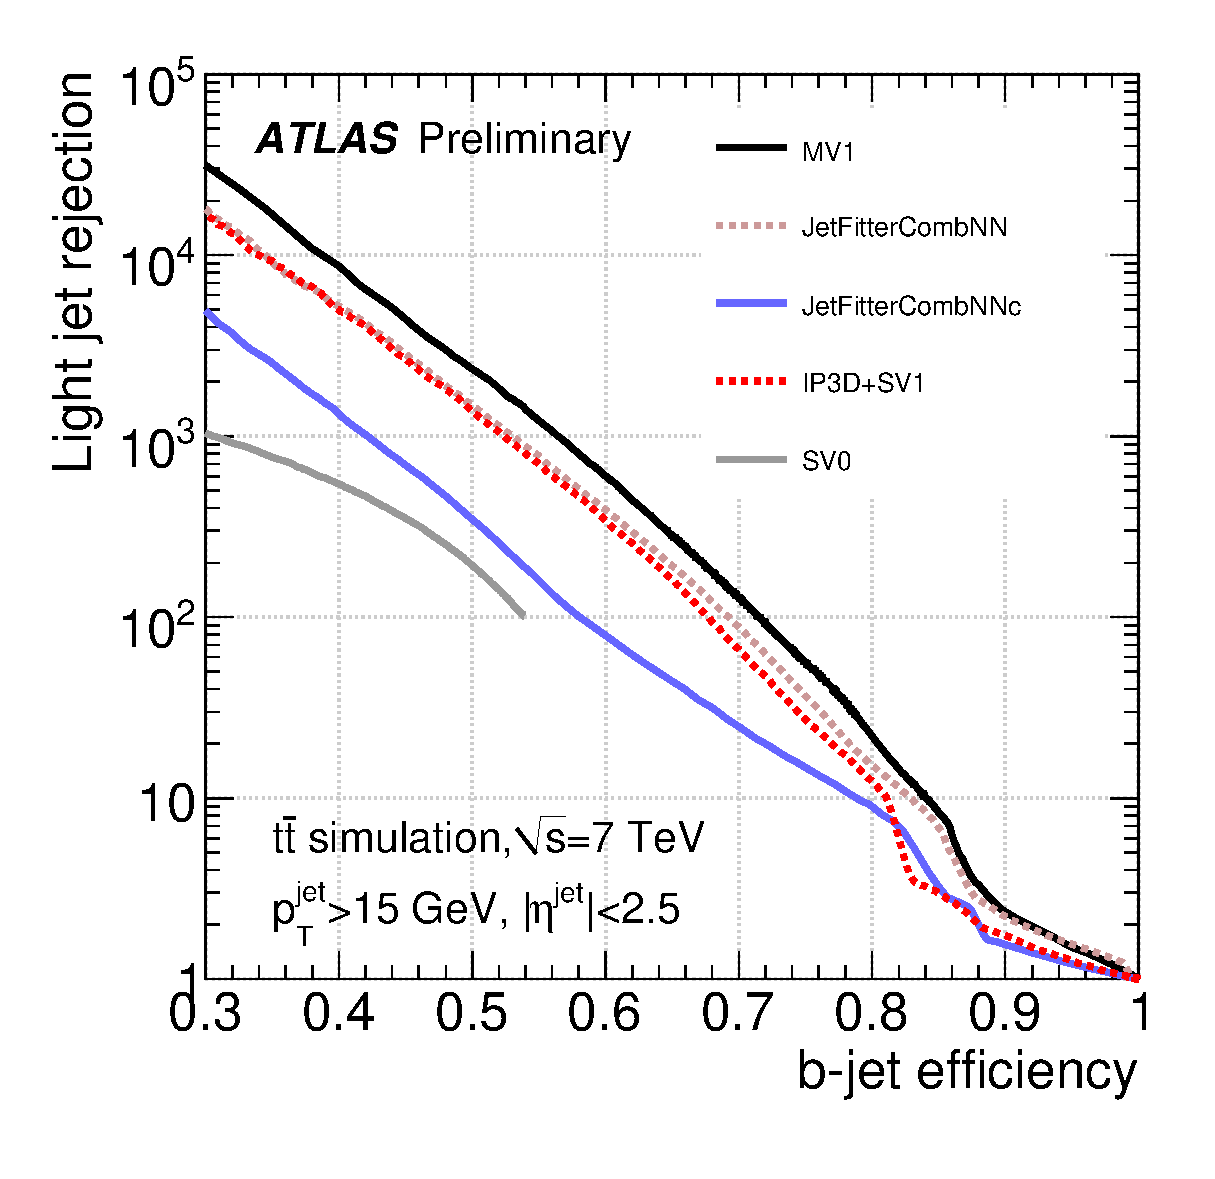
\includegraphics[width=0.99\textwidth]{Objects/Figures/fig_01a_bTagging.eps}
\caption{}
\end{subfigure}
\begin{subfigure}[]{0.40\textwidth}
   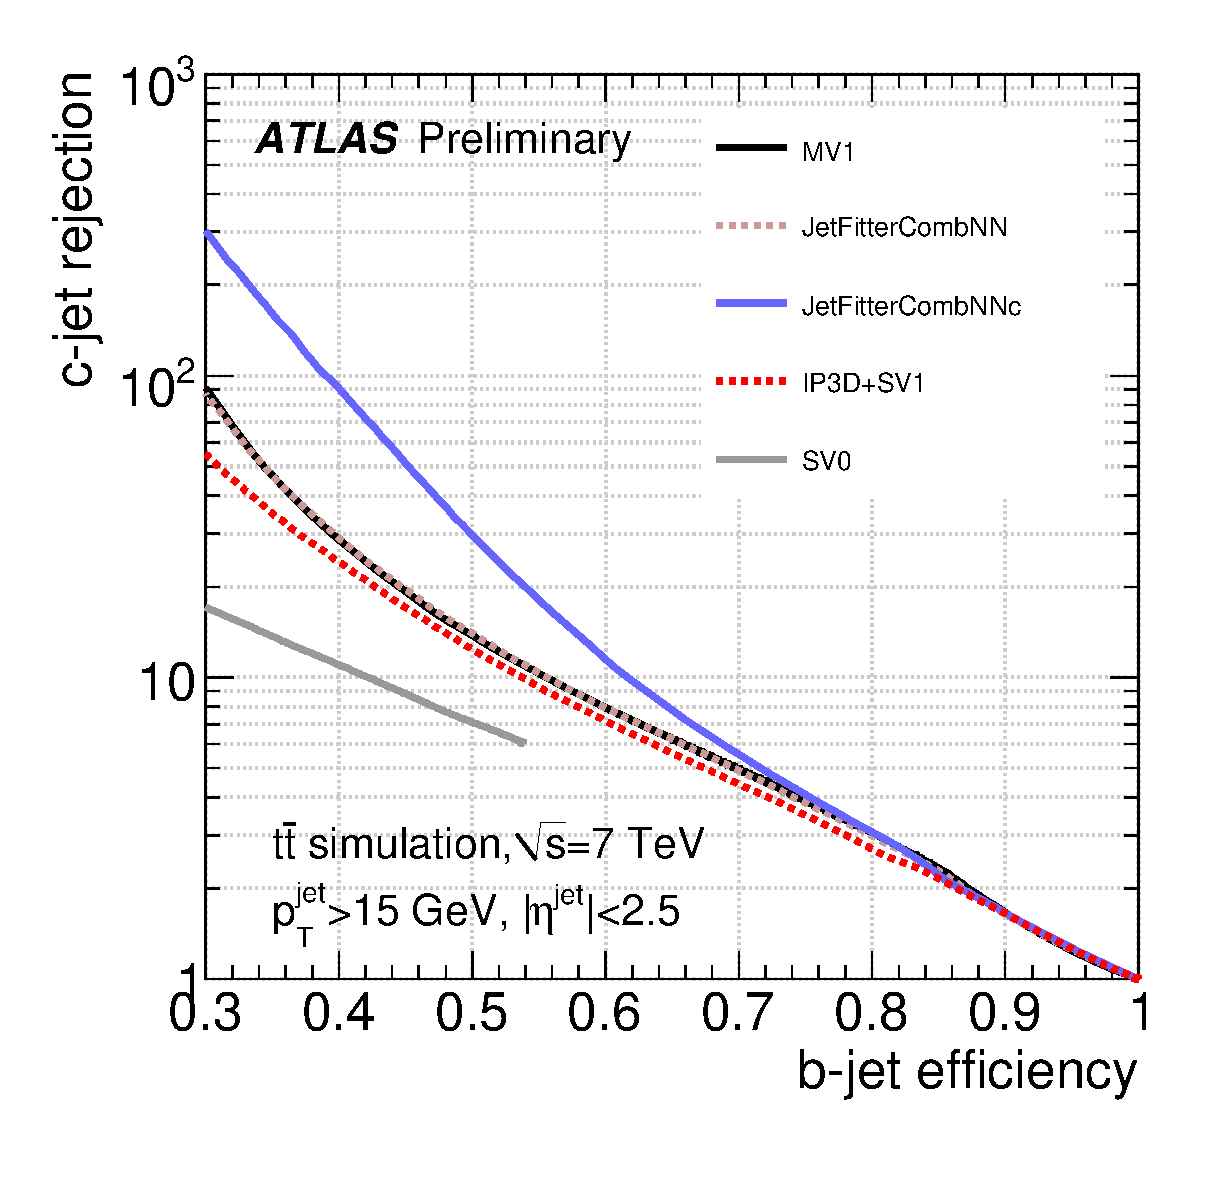
\includegraphics[width=0.99\textwidth]{Objects/Figures/fig_01b_bTagging.eps}
   \caption{}
\end{subfigure}
\caption{ Light-jet rejection (a) and c-jet rejection (b) as a function of the $b$-jet efficiency for different available $b$-tagging algorithms, based on simulated \ttbar\ events~\protect\cite{BTagptrel}.
}
\label{fig:OBbtag}
\end{figure} 

Several operating points have been considered based on the average efficiency of the algorithm on simulated \ttbar\  events. Some of them are listed in table~\ref{tab:OBop}.
The \unit[70]{\%} operating point has been chosen for most of the \ttbar\ based analyses given the good compromise between efficiency and rejection.
Figure~\ref{fig:OBmceff} shows the efficiency, obtained from the simulation, of the \unit[70]{\%} MV1 operating point for $b$-jet, $c$-jet and light-jets as a function of the jet 
\pT\ and $\abseta$. The $b$-tagging efficiency increases at high \pT\ where the identification of displaced vertices is more efficient. The mistag rate is more important for large $\abseta$ values due to the worse track resolution.
\begin{table}[hbt] %%]htb]
\centering     % 1 2 3 4 5
\begin{tabular}{c c c}
\toprule
\toprule
$b$-jet efficiency &  $c$-jet rejection & light-jet rejection \\
\midrule
\unit[50]{\%}		& 13.7 	&  2330 \\ 
\unit[60]{\%}		& 7.9 	&  590 \\ 
\unit[70]{\%}		& 5.0 	&  140  \\
\unit[80]{\%}		& 3.1 	&    25 \\ 
\bottomrule
\bottomrule
\end{tabular}
\caption{The MV1 algorithm operating points and their performance. The $b$-jet efficiency is the average obtained for $b$-jets from a \ttbar\ sample. }
\label{tab:OBop}
\end{table}


\begin{figure}[tb!] %ht!p
\centering
%%%%\begin{adjustwidth}{-0.8cm}{}
\begin{subfigure}[t]{0.45\textwidth}
   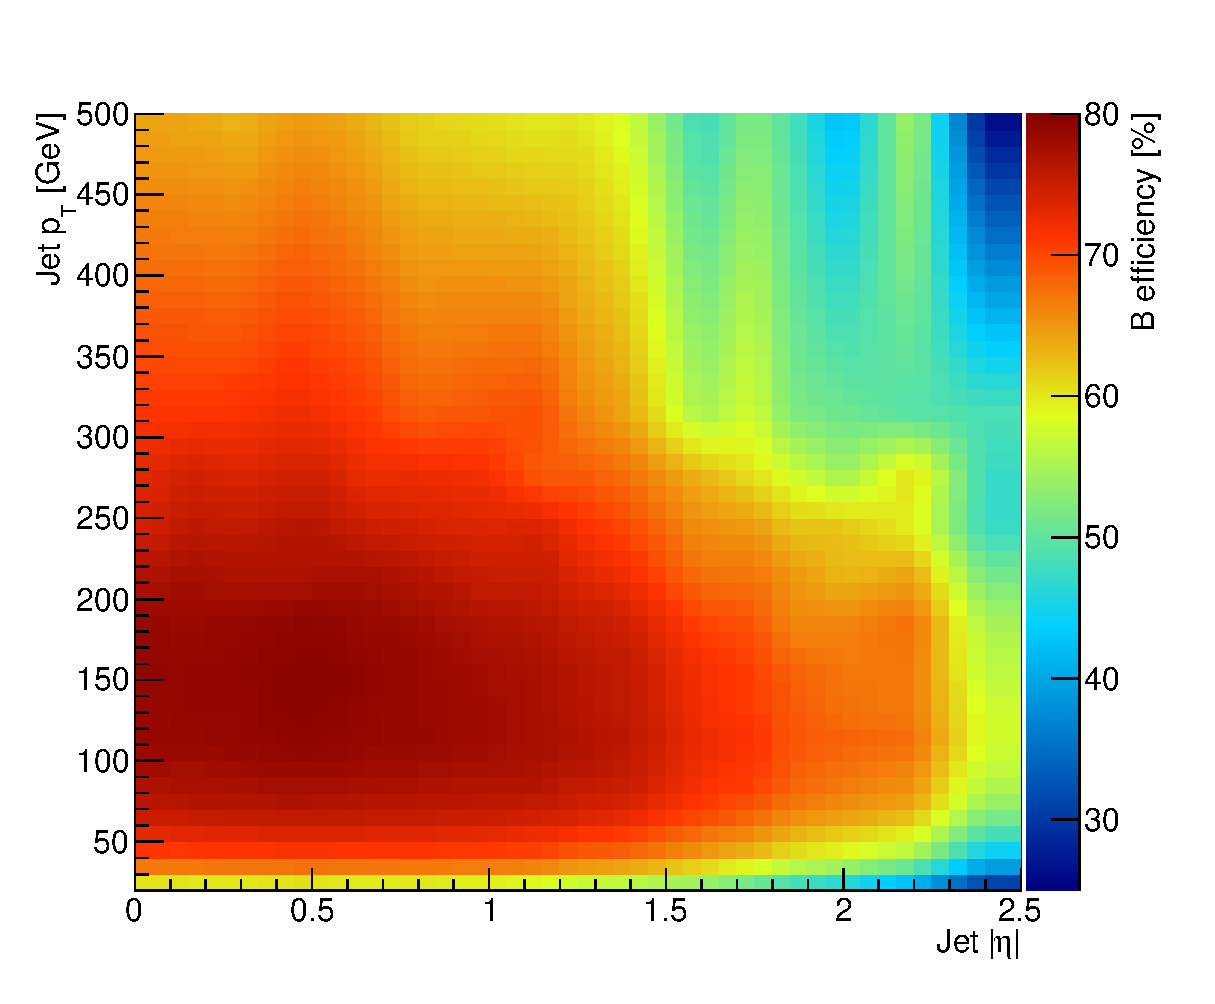
\includegraphics[width=0.99\textwidth]{Objects/Figures/eff_b.eps} %png}
\caption{}
\end{subfigure}
\begin{subfigure}[t]{0.45\textwidth}
   \includegraphics[width=0.99\textwidth]{Objects/Figures/eff_c.eps} %png}
   \caption{}
\end{subfigure}
\begin{subfigure}[t]{0.45\textwidth}
   \includegraphics[width=0.99\textwidth]{Objects/Figures/eff_u.eps} %png}
   \caption{}
\end{subfigure}
%%\end{adjustwidth}
\caption{$b$-tagging efficiency for the MV1 70\% operating point as a function of the jet \pT\ and $|\eta|$. Efficiencies are shown separately for (a) $b$-jets, (b) $c$-jets and (c) light-jets from simulated \ttbar\ events. }
\label{fig:OBmceff}
\end{figure} 


\subsection{$b$-tagging calibration}
The efficiency of each operating point has been calibrated in data using samples enriched in $b$-jets, $c$-jets and light jets respectively.
The result is presented in terms of scale factors, SF$=\epsilon_{\rm data} / \epsilon_{\rm MC}$. This allows correcting for mis-modeling in the input variables used in the $b$-tagging algorithms.
Different methods have been used to derive the respective calibrations:

%Several methods were used to calibrate the efficiency on a $b$-jet enriched samples, they can be divided into two different families according to the sample they use.
%
%Di-jet based calibrations rely on semileptonic $b$-hadron decays identified through the presence of a ``soft'' muon inside the jet. 
%The $\pT^{\rm rel}$ method exploits the fact that the relative momentum of the muon with respect to the jet axis is larger for a jet originating from a $b$-quark. A template fit procedure is performed to extract the fraction of $b$-hadrons before and after the application of the tag requirement to the jet.
%The system8 method combines three uncorrelated selection criteria to construct a system of eight equations based on the number of events surviving any given subset of these criteria.
%The first criterion is the selection of the $b$-tagging algorithm under consideration, the second requires that the ``soft'' muon has a $\pT^{\rm rel} > 700 \MeV$ and the third criterion demands the presence of another jet opposite the selected one that contains a well identified secondary vertex.
%Di-jet based calibrations were the first methods used in the 2010 and 2011 data taking. They cover the low/medium \pT\ range for jets since at high jet \pT\ ( $>200 \GeV$) other than reduction of the data statistics, the method becomes less performing due to the similarity of the $\pT^{\rm rel}$ distributions.
%but the statistic in data drastically reduce at high jet 
%\ttbar-based calibrations exploit the presence of $b$-jets produced in a \ttbar\ decay. 
%As will be discussed later in this document, a \ttbar\ enriched sample can be easily obtained with a l+jets or di-lepton selection 
%and a specific kinematic selection allows identifying a $b$-jet sample with a purity ranging from 50\% to 90\%. 
%\ttbar-based calibrations have become a very precise tool especially for the 2012 dataset given the large amount of collected \ttbar\ events. 

The $b$-jet calibration used for the analyses in this dissertation is derived on a high-purity sample of $b$-jets that can be obtained from dileptonic \ttbar\ events.
The calibration is based on a likelihood approach which uses correlated information from multiple jets in the event~\cite{BTagSF}, and 
it achieves a precision of a few \% for jet \pT\ ranging between 30 and 200 \GeV. 
%Nevertheless a correct use in a \ttbar\ analysis requires some additional care in order to avoid a re-use of the same data sample as well as double counting of systematic uncertainties.
%In this respect di-jet based calibrations are easier to use in a \ttbar\ analysis since the analysis sample and the sample used for calibration are independent and the two analyses have very different sources of systematic uncertainties.
Since the calibration has been derived using a dileptonic \ttbar\ sample, no overlap of data events 
exists with analyses performed in the single-lepton final state.

%re-write the formula in atlas-style
The tagging calibration on $c$-quarks has been derived by reconstructing $D$-mesons within a jet from the decay chain $D^{*+} \rightarrow D^{0} (\rightarrow K^{-}\pi^{+})\pi^{+}$~\cite{CTagSF}.
%The fraction of $D^{*+}$ originating from hadronic $b$ decays has been extracted by a fit to the pseudo-proper time of the selected candidates.
%The $b$-tagging efficiency for $c$-quark initiated jets has thus been measured by comparing the corrected yields of $D^*$ mesons before and after the application of the MV1 cut.
%In 2012, a correction factor covering the extrapolation from semileptonic $D$-mesons decay to the inclusive sample is also applied~\cite{CTagSFextr}. 
%Uncertainties on the data/MC scale factors for the 70\% MV1 operating point span in the range of 10 \% to 20 \% .

For the mis-tag rate, the ``negative tag'' method is used~\cite{LTagSF}. Light-jets are expected to have a rather symmetric track impact parameter or vertex decay length significance distribution. 
The performance of the tagger is evaluated by using tracks (vertices) with negative impact parameter (decay length significance) and reversing their sign within the algorithm.
%Light jets are expected to have a rather symmetric track impact parameter or vertex decay length significance distribution\footnote{sources of asymmetries like long lived meson decays are taken into account with a correction factor} where large absolute values could arise due to the finite resolution of the tracker.
%The negative side of this distribution is then used as an estimate for the positive side distribution since in the former the shape of the distribution is rather similar between light, $b$ and $c$-jets thus reducing the effect of contaminations.
%%suffers from a much lower contamination from b and c-jets.
%The performance of the tagger is evaluated by using tracks/vertices with negative impact parameter/decay length significance and reverse their sign within the algorithm.
%For the MV1 70\% operating point, the uncertainties range between 25\% and 35\% as a function of \pT\ and $|\eta|$ of the jet.

%\cor{Here the 'problem' is that I don't know which SF/calibration we are going to use: ttbar-based SF or the pure self-calibration. I need to expand the concept where it will be clear how the final analysis will apply the calibration.}
Scale factors as a function of jet \pT\ for $b$-jet, $c$-jet and light-jets are reported in figure~\ref{fig:OBbtagsf}.
The scale factors are applied to MC samples as event weight corrections.
For each jet tagged by the $b$-tagging algorithm, a weight equal to the $b$-tagging scale factor, SF, of the corresponding jet flavor is considered.
If a jet fails the $b$-tagging criterion, a weight corresponding to $(1-{\rm SF}\cdot \epsilon_{\rm MC})/(1-\epsilon_{\rm MC})$ is assumed.  
The individual jet weights for all the selected jets are multiplied in order to obtain an event-level weight.

\begin{figure}[tb!]
\centering
%%\begin{adjustwidth}{-0.4cm}{} %%-0.5
\begin{subfigure}[t]{0.45\textwidth}
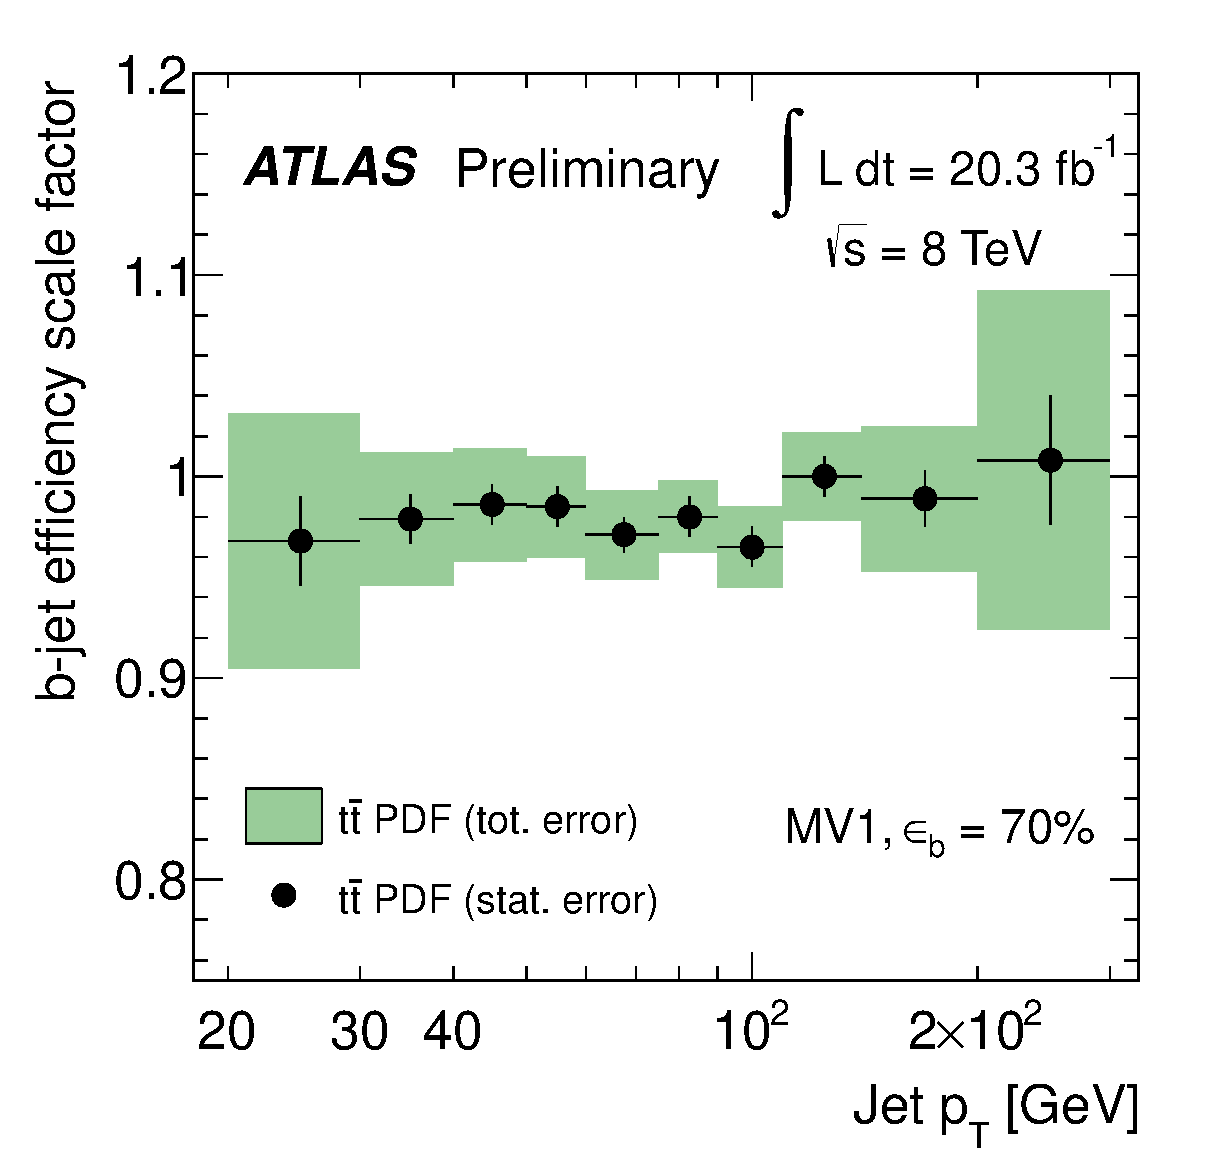
\includegraphics[width=0.99\textwidth, height=4.4cm, keepaspectratio=false]{Objects/Figures/fig_02b_B_SF.eps}
\caption{}
\end{subfigure}
\begin{subfigure}[t]{0.45\textwidth}
  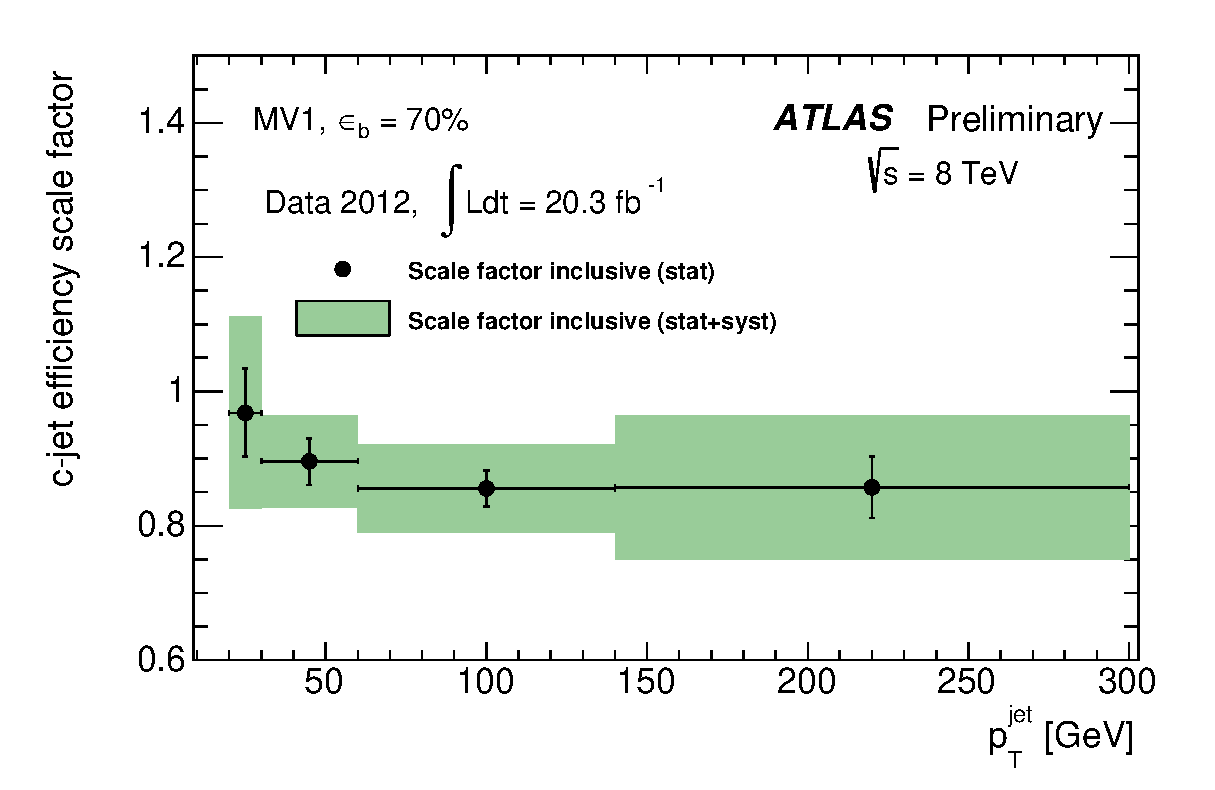
\includegraphics[width=0.99\textwidth]{Objects/Figures/fig_06_C_SF.eps}
   \caption{}
\end{subfigure}
\begin{subfigure}[t]{0.45\textwidth}
  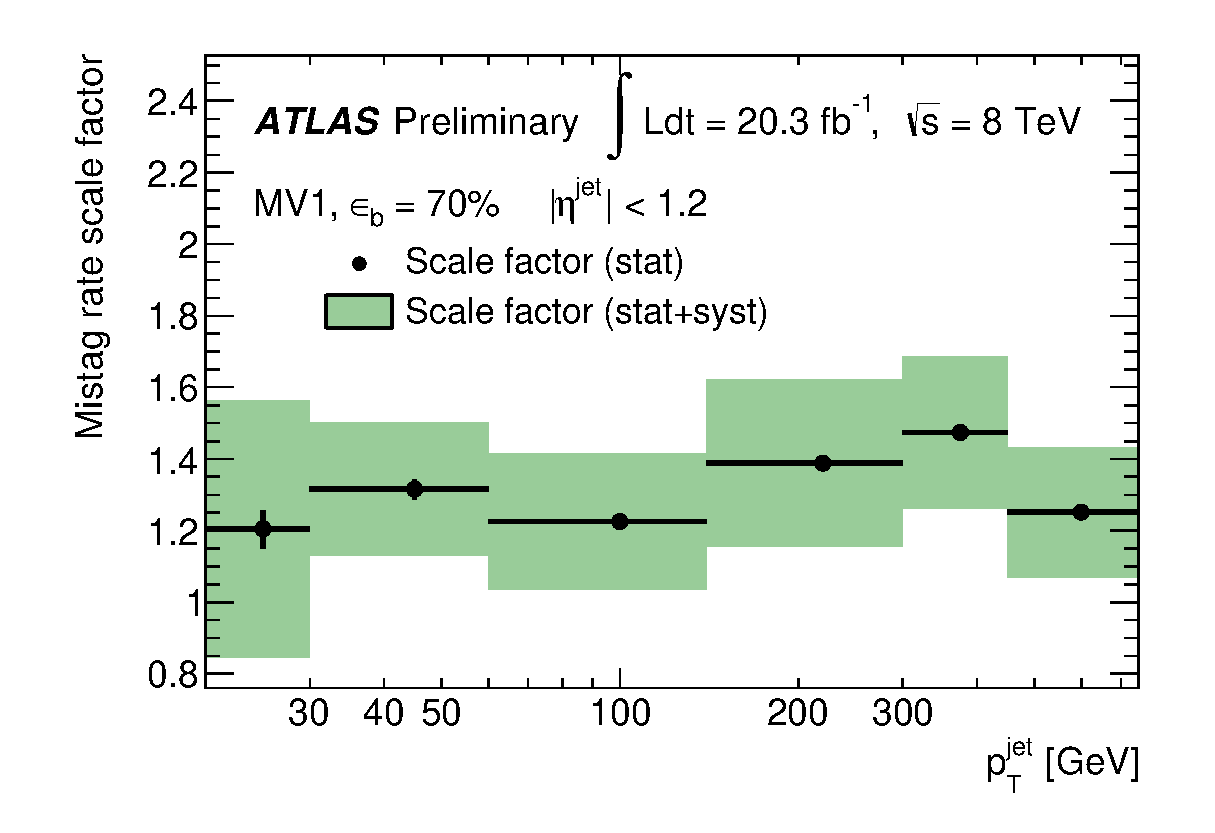
\includegraphics[width=0.99\textwidth]{Objects/Figures/fig_08c_L_LB_SF.eps}
   \caption{}
\end{subfigure}
\begin{subfigure}[t]{0.45\textwidth}
  \includegraphics[width=0.99\textwidth]{Objects/Figures/fig_08d_L_EB_SF.eps}
   \caption{}
\end{subfigure}
%%\end{adjustwidth}
\caption{ Data/MC scale factor for the tagging efficiency of (a) $b$-jets, (b) $c$-jets and (c) light jets in the central and (d) forward region with the \unit[70]{\%} MV1 operating point. The total uncertainty is shown as well as the statistic components.
Scale factors are measured as a function of jet \pT\ and, in the case of mistag rate, the result for the two $|\eta|$ bins are shown.}
\label{fig:OBbtagsf}
\end{figure} 


The determination of the $b$-tagging scale factors is affected by multiple systematic uncertainties. In order to propagate those into the scale factors in a manageable way the diagonalization method is used.
The covariance matrix of the scale factors in the different jet \pt\ bins is diagonalized. The eigenvectors with their respective eigenvalues represent the variations which are needed to describe the $b$-tagging efficiency uncertainty induced on the analysis.
Since these variations result from the diagonalization of the covariance
matrix, they can be considered as independent variations and are treated in the
analysis as uncorrelated uncertainties.
After diagonalization, a total of six eigenvectors are considered to describe the systematic uncertainties related to the $b$-tagging calibration. The same procedure is performed to derive four (twelve) eigenvectors on the $c$-tagging (mistag) calibration.

The $b$-tagging calibration for $b$-jets and $c$-jets only extends to \unit[300]{\gev} in jet \pT, with the light-jet calibration extending to \unit[750]{\gev}. A MC-based analysis is used to assess an extrapolation uncertainty on the $b$-tagging efficiency from the last calibrated \pT\ bin up to \unit[1200]{\gev}, to judge how systematic effects could impact the higher \pT\ jets compared to the last calibrated bin. An additional uncertainty is included for jets with \pt\ above the calibrated range.


\section{Missing transverse energy}
Particles like neutrinos and other neutral weakly-interacting particles predicted in BSM scenarios escape ATLAS undetected, thus creating an apparent imbalance of the measured momentum in the transverse plane.
The missing transverse momentum, $\ptmiss$, is obtained from the negative vector sum of the \pt\ of all particles detected in a $\pp$ collision.
The magnitude of this vector is the missing transverse energy, $\met$.

The $\met$ reconstruction~\cite{TheATLAScollaboration:2013oia} includes contributions from energy deposits in the calorimeters and muons reconstructed in the muon spectrometer.
\begin{equation}
  E_{\rm{x(y)}}^{\rm{miss}} =E_{\rm{x(y)}}^{\rm{miss,calo}} + E_{\rm{x(y)}}^{\rm{miss,muon}}
  \label{eq:MET_definition}
\end{equation}

Isolated muons are measured by combining the information in the muon spectrometer and the inner detector. %~\ref{subsec:Muons}
In the case of non-isolated muons, the momentum measurement is taken from the muon spectrometers only and an additional term for the energy deposit in the calorimeter is considered.

Energy deposits in calorimeter cells are associated with identified physics objects and are considered in the calculation with the calibration of these associated objects.
Double counting is avoided by considering physics objects in a specific order: electrons, jets and muons. 
\begin{equation}
  E_{\rm{x(y)}}^{\rm{miss,calo}} =E_{\rm{x(y)}}^{\rm{miss,e}}+E_{\rm{x(y)}}^{\rm{miss,jet}}+\left(E_{\rm{x(y)}}^{\rm{miss,muon-calo}}\right)+E_{\rm{x(y)}}^{\rm{miss,soft-jet}}+E_{\rm{x(y)}}^{\rm{miss,cell-out}}
  \label{eq:METcalo_definition}
\end{equation}


The $E_{\rm{x(y)}}^{\rm{miss,soft-jet}}$ term is built considering jets with $10 \GeV < \pT < 20 \GeV$, calibrated at the LCW scale without jet area correction.
The $E_{\rm{x(y)}}^{\rm{miss,cell-out}}$ term collects all the deposits that are not associated with any physics object.
%Both jet terms do not take into account a jet if its JVF is equal to 0. 
%The muon term ($E_{\rm{x(y)}}^{\rm{miss,muon}}$) contains the combined muon momenta; calorimetric cells associated to the muon energy loss are then excluded.

The effects of systematic uncertainties in the \met\ computation are divided into two main sources: uncertainties affecting high-\pT\ objects and uncertainties affecting the soft-jet and the cell-out terms.
For the former, systematic uncertainties on the physics object calibrations are directly translated into the missing transverse energy computation through equation~\ref{eq:MET_definition}.
The uncertainties on $\ET^{\rm{miss,soft-jet}}$ and $\ET^{\rm{miss,cell-out}}$ are considered to be fully correlated, and they are  evaluated in events with no real source of \met\, such as $Z\rightarrow \mumubar$ events with no jets with $\pT>20 \GeV$.
An uncertainty of 2.3\% and 3.6\% has been assigned respectively to the resolution and scale of both terms~\cite{TheATLAScollaboration:2013oia}.

\clearpage
\bibliographystyle{Bibliography/atlasnote}
\bibliography{Bibliography/myBib}
